\chapter{Model validation}
The model was validated comparing the results with either behavioural circuit simulations and experimental circuits.  Because the proposed method has the goal to model losses produced by the charge transfer between capacitors and conductance through resistive elements (switches and parasitics), simulations with a behavioral simulator only take into account these two sources of losses, enabling a fair comparison to validate the proposed model.  Nevertheless, an experimental converter was specifically build with the only propose to validate measure and validate the model. The converter was designed to mitigate any other source of loss not included in the model, such as switching losses, driving losses, etc. These other loss mechanisms can be added to the model as described in~\cite{Seeman:EECS-2009-78}; however, they are out of the scope of the model presented in the previous chapter.

This chapter is divided in two sections. The first section validates the mode for single output SCC, based on simulations the results are presented for both the common \emph{dc}-output and the \emph{pwm}-outputs.  The second section validates the multiple output model using both circuit simulations and an experimental setup.

\section{Single output SCC}
The validation of the modeling for single output SCC has been done for the two types of output nodes: \emph{dc} and \emph{pwm}. In both cases the validation is performed comparing the predicted $r_{scc}$ of the model with the measured values from a the behavioural circuit simulator PLECS. In the case of the case of the \emph{dc}-node the results are also compared with the original charge flow analysis since it was the currently used methodology.

The same 3:1 Dickson was used as a test circuit. First connecting the load to the \emph{dc}-node as shown in Figure~\ref{fig:3_1_hscc_exp_a}, and second connecting the load to the \emph{pwm}-node as shown in Figure~\ref{fig:3_1_hscc_exp_b}. In both cases the load was emulated with a constant current source. In both simulations the design parameters were kept the same as defied in Table~\ref{tab:sim_values}.

\begin{table}[h]
\centering
\caption{3:1 Dickson design parameters used in PLECS simulator.}
\section{\label{tab:sim_values}}
\renewcommand{\arraystretch}{1.5}% Wider
\begin{tabular}{l | c  }
 Parameter  &  Value  \\
 \midrule
 $v_{in}$   & 10V \\
 $r_{on}$   & 100$m\Omega$ \\
 $c_x$      & 100$nF$\\
 $\eta$\footnote{Efficiency} & 95$\%$
\end{tabular}
\end{table}

The load current $i_{out}$ was adjusted in each simulation depending on the operation point of the converter, keeping the efficiency to $\eta=95\%$, by using the following expression
\begin{equation}
    i_{out}=m_x~v_{src}\frac{1-\eta}{r_{scc,mdl}},
\label{eq:iout_eff}
\end{equation}
where $m_x$ is the conversion ratio for the given output and $r_{scc,mdl}$ is the predicted output resistance by the model. Fixing the efficiency, guarantees the same average output voltage across all the simulations, since rearranging~\eqref{eq:eff_vo} yields
\begin{equation}
    v_{out}=m_x~v_{src}~\eta.
\label{eq:vout_eff}
\end{equation}
Using high enough efficiency values prevents the load to fully discharge the capacitors of the converter, avoiding to bring the converter in an undesired operating regime.


\subsection{Measuring $r_{scc}$ from a SCC}
\begin{figure}[!h]
\centering
\ctikzset { bipoles/length=1cm}
\begin{circuitikz}[american,scale=0.65]
\draw
    (2.5,0) to[short]
    (-1.5,0) to[V = $v_{src}$](-1.5,3) -- (2.5,3)
    %(-1.5,3) to[ammeter,l=$i_{in}$]  (1,3) -- (2.5,3)
    (1,3) to[voltmeter,l_=$v_{in}$] (1,0);


\draw [thick]
    (2.5,-0.5) --
    (2.5,3.5)  --
    (5.5,3.5)  --
    (5.5,-0.5) --
    (2.5,-0.5);

\draw (4,1.5) node[align=center]{SCC \\ U.T.} ;

\draw
    (5.5,3) --
    (7,3) to[ammeter,l=$i_{out}$]
    (9.5,3) to[gswitch,l=$s_1$]  (10,3) -- (10.5,3) to[I,l = $i_{load}$]
    (10.5,0) -- (5.5,0)
    (7,3) to[voltmeter,l^=$v_{out}$] (7,0);
\end{circuitikz}
\caption{Experimental arrangement used to test and measure the characteristics of an SCC. }
\label{fig:rscc_exp_setup}
\end{figure}
Figure~\ref{fig:rscc_exp_setup} shows the configuration used to measure the $r_{scc}$ in the circuit simulator. By measuring the input and outputs currents and voltages the $r_{scc}$ is computed in two steps, operating the converter with the same values of $f_{sw}$ and $D$:
\begin{enumerate}
  \item Operating with no load ($s_1$ open), the \emph{target voltage} ($v_{trg}$) and the conversion ration $m$ are determined,
      \begin{align}
        v_{trg} & = v_{out},\label{eq:vtrg}\\
        m & = \frac{v_{out}}{v_{in}}.
        \label{eq:vtrg_m}
      \end{align}

  \item Loading the converter with constant current ($s_1$ closed),  $r_{scc}$ is computed using~\eqref{eq:vtrg},
      \begin{equation}
        r_{scc} = \frac{v_{trg} - v_{out}}{i_{out}}.
        \label{eq:rscc_m}
      \end{equation}
\end{enumerate}

\subsection{ Fixed \emph{dc}-output}
\begin{SCfigure}[][!h]
    \ctikzset { bipoles/length=1cm}
    \centering
    \begin{circuitikz}[american ,scale=0.6]
    \draw
            %Input Supply
            %(0,0)  to[V=$v_{src}$]
            %Draw Switches
            %(0,10)  --
            (5,10.3) node[anchor=south] {$v_{src}$}
            (5,10) node[rground, yscale=-1] {}
            to[gswitch=$s_1$] %S1
            (5,8)   to[gswitch=$s_2$] %S2
            (5,6)   to[gswitch=$s_3$] %S3
            (5,4) --
            %left branch
            (3,4)   to[gswitch=$s_7$]
            (3,2)   to[gswitch=$s_6$]
            (3,0);

    \draw   %right branch
            (5,4) --
            (7,4)   to[gswitch,l_=$s_4$]
            (7,2)   to[gswitch,l_=$s_5$]
            (7,0) -- (3,0);


    \draw %Capacitor C1
           (3,2) -- (2,2) -- (2,4)
            to[pC,l_=$c_1$] (2,8) --
           (5,8);

    \draw %Capacitor C2
           (7,2) --
           (8.25,2) -- (8.25,3.5)  to[pC,l^=$c_2$] (8.25,6) --
           (5,6);

    \draw %Capacitor C3
           (5,0) node[sground] {} to[pC,l_=$c_3$] (5,4);

     %\draw (7,4) to[short,-o] (10,4) node[anchor=west] {};

     %\draw (9,6) to[open,v^=$v_{1}$] (9,0);
     \draw (5,4)  --([hs]8.25,4 |- 5,4) arc(180:0:\radius) to[short] (9.5,4) to[I,l^=$i_{out}$] (9.5,0) |- (5,0);
     \end{circuitikz}
\caption{3:1 Dickson circuit used to validate the model accuracy in the prediction of  $r_{scc}$ for the \emph{dc}-node.}
\label{fig:3_1_hscc_exp_b}
\end{SCfigure}

Figure~\ref{fig:exp_rscc_dc_node_dx} shows $r_{scc}$ for a sweep in duty cycle ($D$) between $10\%$ and $9\%$, simulated at four different frequencies: 100kHz, 1MHz, 10MHz and 100MHz; thus operating the converter between the different switching limits (SSL and FSL).

The square markers are the measured resistance from the PLECS simulation, the solid black lines with markers: circle, plus and times, are the results of the model using the different approximations respectively: Original, Markowski and modified Markowski previously described in Section~\ref{ch:rscc_apprx}. The grey markers are the relative error between the model results and the PLECS simulation.  The two grey lines belong to the results of the previous modeling methods, the dashed line corresponds to the results of the original charge flow method proposed  by~\citeauthor{95Makowski} in~\citeyear{95Makowski}, and the dotted line is a posterior addition to the method, proposed by~\citeauthor{2013Breussegem:c_out} in~\cite{2013Breussegem:c_out} that includes the effects of the output capacitor.

\begin{figure}[!h]

\centering
    \begin{subfigure}{\textwidth}
        \parbox[c]{.03\linewidth}{\subcaption{}\label{fig:exp_rscc_dc_node_100kHz}}
        \hspace{.02\linewidth}
        \parbox[c]{.95\linewidth}{
        \centering
        % This file was created by matlab2tikz.
%
%The latest updates can be retrieved from
%  http://www.mathworks.com/matlabcentral/fileexchange/22022-matlab2tikz-matlab2tikz
%where you can also make suggestions and rate matlab2tikz.
%

\begin{tikzpicture}
\pgfplotsset{
    width=9cm,
    height=2.5cm,
    scale only axis,
    xlabel near ticks,
    ylabel near ticks,
    enlarge y limits={0.2},
    legend style={
                legend columns = 3,
                at={(0.5,1.075)},
                anchor=south,
                draw=none,
                font=\small,
                column sep=2ex,
                legend cell align=left},
}

\begin{axis}[%
    axis x line*=bottom,
    axis y line*=left,
    %xlabel= {duty cycle},
    ylabel= {$r_{scc}~[\Omega]$},
    yticklabel style={text width=2em,align=right},
    ]

    \addplot [semithick,mark=square,only marks,white]
      table[y=y1] {./3_modeling/rx_sw_dx_O2.dat};\label{pl_PLECS_hidden}

    \addplot [semithick,mark=square,only marks]
      table[y=y1] {./3_modeling/rx_sw_dx_O2.dat};\label{pl_PLECS}


    \addplot [semithick,smooth,mark=o,mark repeat=10]
      table [y=y1] {./3_modeling/rm1_sw_dx_O2.dat};\label{pl_MDL_JD}

    \addplot [semithick,smooth,mark=+,mark repeat=10]%black!66]
      table [y=y1] {./3_modeling/rm2_sw_dx_O2.dat};\label{pl_Makw}

    \addplot [semithick,smooth,mark=x,mark repeat=10]%black!33]
      table [y=y1] {./3_modeling/rm3_sw_dx_O2.dat};\label{pl_Makw rec}

    \addplot [semithick,smooth,dashed,black!75]
      table [y=y1] {./3_modeling/rm1_ms_sw_dx_O2.dat};\label{pl:95Makw}

    \addplot [semithick,smooth,dotted,black!75]
      table [y=y1] {./3_modeling/rx_ST_sw_dx_1Co.dat};\label{pl:Stey}



\end{axis}

\begin{axis}[%
    axis y line*=right,
    axis x line=none,
    ylabel = {$\epsilon_r~[\%]$},
    yticklabel pos=right,
    yticklabel style={text width=2em,align=left},
    ]
    \addlegendimage{/pgfplots/refstyle=pl_PLECS}\addlegendentry{PLECS}
    \addlegendimage{/pgfplots/refstyle=pl_MDL_JD}\addlegendentry{This Work}

    \addplot [semithick,mark=o,only marks,black!60]
      table [y=y1] {./3_modeling/err1_sw_dx_O2.dat};
    \addlegendentry{ $\epsilon_r$ (Rel. Error)}


    \addlegendimage{/pgfplots/refstyle=pl_PLECS_hidden}\addlegendentry{\color{white}PLECS}
    \addlegendimage{/pgfplots/refstyle=pl_Makw}\addlegendentry{Makowski}
    \addplot [semithick,mark=+,only marks,black!60]
      table [y=y1] {./3_modeling/err2_sw_dx_O2.dat};
    \addlegendentry{$\epsilon_r$ \color{white}(Rel. Error) }

    \addlegendimage{/pgfplots/refstyle=pl_PLECS_hidden}\addlegendentry{\color{white}PLECS}
    \addlegendimage{/pgfplots/refstyle=pl_Makw rec}\addlegendentry{*Mak. }
    \addplot [semithick,mark=x,only marks,black!60]
      table [y=y1] {./3_modeling/err3_sw_dx_O2.dat};
    \addlegendentry{$\epsilon_r$ \color{white}(Rel. Error)}

    \addlegendimage{/pgfplots/refstyle=pl_PLECS_hidden}\addlegendentry{\color{white}PLECS}
    \addlegendimage{/pgfplots/refstyle=pl:95Makw}\addlegendentry{95Makowski.}
    \addlegendimage{/pgfplots/refstyle=pl:Stey}\addlegendentry{Steyaert}


\end{axis}
\end{tikzpicture}




}
    \end{subfigure}

    \begin{subfigure}{\textwidth}
        \parbox[c]{.03\linewidth}{\subcaption{}\label{fig:exp_rscc_dc_node_1MHz}}
        \hspace{.02\linewidth}
        \parbox[c]{.95\linewidth}{
        \centering
        % This file was created by matlab2tikz.
%
%The latest updates can be retrieved from
%  http://www.mathworks.com/matlabcentral/fileexchange/22022-matlab2tikz-matlab2tikz
%where you can also make suggestions and rate matlab2tikz.
%

\begin{tikzpicture}
\pgfplotsset{
    width=9cm,
    height=2.5cm,
    scale only axis,
    ylabel near ticks,
    enlarge y limits={0.2},
    xlabel near ticks,
    ylabel near ticks,
}
\begin{axis}[%
axis x line*=bottom,
axis y line*=left,
xlabel= {duty cycle},
ylabel= {$r_{scc}~[\Omega]$},
yticklabel style={text width=2em,align=right}
]

    \addplot [semithick,mark=square,only marks]
      table[y=y4] {./3_modeling/rx_sw_dx_O2.dat};\label{pl_PLECS}
    \addplot [semithick,smooth,black]
      table [y=y2] {./3_modeling/rm1_sw_dx_O2.dat};\label{pl_MDL}
    \addplot [semithick,smooth,black!66]
      table [y=y2] {./3_modeling/rm2_sw_dx_O2.dat};
    \addplot [semithick,smooth,black!33]
      table [y=y2] {./3_modeling/rm3_sw_dx_O2.dat};
    
    \addplot [semithick,smooth,black,dashed]
      table [y=y2] {./3_modeling/rm1_ms_sw_dx_O2.dat};\label{pl_MDL}

\end{axis}

\begin{axis}[%
    axis y line*=right,
    axis x line=none,
    ylabel = {$\epsilon_r~[\%]$},
    yticklabel pos=right,
    yticklabel style={text width=2em,align=left},
    ]

    \addplot [semithick,mark=star,only marks,black]
    table [y=y4] {./3_modeling/err1_sw_dx_O2.dat};

    \addplot [semithick,mark=star,only marks,black!66]
    table [y=y4] {./3_modeling/err2_sw_dx_O2.dat};

    \addplot [semithick,mark=star,only marks,black!33]
    table [y=y4] {./3_modeling/err3_sw_dx_O2.dat};

\end{axis}
\end{tikzpicture}
}
    \end{subfigure}

    \begin{subfigure}{\textwidth}
        \parbox[c]{.03\linewidth}{\subcaption{}\label{fig:exp_rscc_dc_node_10MHz}}
        \hspace{.02\linewidth}
        \parbox[c]{.95\linewidth}{
        \centering
        % This file was created by matlab2tikz.
%
%The latest updates can be retrieved from
%  http://www.mathworks.com/matlabcentral/fileexchange/22022-matlab2tikz-matlab2tikz
%where you can also make suggestions and rate matlab2tikz.
%

\begin{tikzpicture}
\pgfplotsset{
    width=9cm,
    height=2.5cm,
    scale only axis,
    ylabel near ticks,
    enlarge y limits={0.2},
    xlabel near ticks,
    ylabel near ticks,
}
\begin{axis}[%
axis x line*=bottom,
axis y line*=left,
xlabel= {duty cycle},
ylabel= {$r_{scc}~[\Omega]$},
yticklabel style={text width=2em,align=right},
]

    \addplot [semithick,mark=square,only marks]
      table[y=y7] {./3_modeling/rx_sw_dx_O2.dat};\label{pl_PLECS}
    \addplot [semithick,smooth,black]
      table [y=y3] {./3_modeling/rm1_sw_dx_O2.dat};\label{pl_MDL}
    \addplot [semithick,smooth,black!66]
      table [y=y3] {./3_modeling/rm2_sw_dx_O2.dat};
    \addplot [semithick,smooth,black!33]
      table [y=y3] {./3_modeling/rm3_sw_dx_O2.dat};
    
    \addplot [semithick,smooth,black,dashed]
      table [y=y3] {./3_modeling/rm1_ms_sw_dx_O2.dat};\label{pl_MDL}

\end{axis}

\begin{axis}[%
axis y line*=right,
axis x line=none,
ylabel = {$\epsilon_r~[\%]$},
yticklabel pos=right,
yticklabel style={text width=2em,align=left},
]

    \addplot [semithick,mark=star,only marks,black]
    table [y=y7] {./3_modeling/err1_sw_dx_O2.dat};

    \addplot [semithick,mark=star,only marks,black!66]
    table [y=y7] {./3_modeling/err2_sw_dx_O2.dat};

    \addplot [semithick,mark=star,only marks,black!33]
    table [y=y7] {./3_modeling/err3_sw_dx_O2.dat};

\end{axis}
\end{tikzpicture}
}
    \end{subfigure}

    \begin{subfigure}{\textwidth}
        \parbox[c]{.03\linewidth}{\subcaption{}\label{fig:exp_rscc_dc_node_100MHz}}
        \hspace{.02\linewidth}
        \parbox[c]{.95\linewidth}{
        \centering
        % This file was created by matlab2tikz.
%
%The latest updates can be retrieved from
%  http://www.mathworks.com/matlabcentral/fileexchange/22022-matlab2tikz-matlab2tikz
%where you can also make suggestions and rate matlab2tikz.
%

\begin{tikzpicture}
\pgfplotsset{
    width=9cm,
    height=2.5cm,
    scale only axis,
    ylabel near ticks,
    enlarge y limits={0.2},
    xlabel near ticks,
    ylabel near ticks,
}
\begin{axis}[%
axis x line*=bottom,
axis y line*=left,
xlabel= {duty cycle},
ylabel= {$r_{scc}~[\Omega]$},
yticklabel style={text width=2em,align=right},
]

\addplot [semithick,mark=square,only marks,forget plot]
  table {./3_modeling/sim_rx_100MHz_O2.dat};

\addplot [semithick,solid,forget plot]
  table {./3_modeling/mdl_rx_100MHz_O2.dat};

%\addplot [semithick,dashed,forget plot]
%  table {./3_modeling/mdl_see_rx_100MHz_O1.dat};

\end{axis}

\begin{axis}[%
axis y line*=right,
axis x line=none,
ylabel = {$\epsilon_r~[\%]$},
yticklabel pos=right,
yticklabel style={text width=2em,align=left},
]

\addplot [semithick,mark=star,only marks,forget plot]
  table {./3_modeling/error_rx_100MHz_O2.dat};


\end{axis}
\end{tikzpicture}
}
    \end{subfigure}

\caption{Equivalent Output Resistance ($r_{scc}$) from the \emph{dc}-node of the converter of Figure~\ref{fig:3_1_hscc_exp_b}. Experimental results (\emph{square marks}) compared with the model (\emph{solid line}) at different switching frequencies ($f_{sw}$): $100kHz$ (\emph{a}) , $1MHz$ (\emph{b}), $10MHz$ (\emph{c}) and $100MHz$ (\emph{d}). Plots are obtained using the presented model using  the different analytical $r_{scc}$ approximations (see~\ref{ch:rscc_apprx}): \emph{black} - Original $u=2$ ,\emph{grey} - Makowski  $u=2.54$, \emph{light grey} - rectified Makowski $u=f(D)$, and using the original charge flow analysis (\emph{dashed line}).}
\label{fig:exp_rscc_dc_node_dx}
\end{figure}

\begin{figure}[!h]
\newcommand\pHeigh{3.25cm}
\newcommand\pWidth{2.5cm}
\centering
    \begin{subfigure}{\textwidth}
       \parbox[b]{.325\linewidth}{
            \raggedright
            % This file was created by matlab2tikz.
%
%The latest updates can be retrieved from
%  http://www.mathworks.com/matlabcentral/fileexchange/22022-matlab2tikz-matlab2tikz
%where you can also make suggestions and rate matlab2tikz.
%

\begin{tikzpicture}
\pgfplotsset{
    width=\pWidth,
    height=\pHeigh,
    scale only axis,
    ylabel near ticks,
    enlarge y limits={0.2},
    xlabel near ticks,
    ylabel near ticks,
    enlarge x limits={0.15},
    every tick label/.append style={font=\footnotesize},
}

\begin{loglogaxis}[
		axis y line*=left,
        axis x line*=bottom,
        xticklabels={,,},
        enlarge y limits={0.1},
        ytick = {1e1,1},
        ylabel= {$ r_{scc} ~ [\Omega] $} ,
        %yticklabel style={xshift=0.5ex},
        title={$c_o= c_{fly}$},
        title style = {
                at ={(0.5,1.1)} },
        legend style={
                legend columns = -1,
                at={(0.5,0.97)},
                anchor=south,
                draw=none,
                font=\tiny,
                column sep=1ex},
        ]


    \addplot [thin,mark=square,only marks,black]
      table [y=y1]{./3_modeling/rx_sw_fsw_1Co.dat};
    \addplot [thin,smooth,black,mark=o,mark repeat=2]
      table [y=y1]{./3_modeling/rx_JD_sw_fsw_1Co.dat};\label{pl_MDL}
    %\addlegendentry{Model};
    \addplot [thin,smooth,mark=+,mark repeat=2]
      table [y=y1]{./3_modeling/rx_MS_sw_fsw_1Co.dat};
    %\addlegendentry{Seeman};
    \addplot [thin,smooth,mark=x,mark repeat=2]
      table [y=y1]{./3_modeling/rx_ST_sw_fsw_1Co.dat};
    %\addlegendentry{Steyaert};


\end{loglogaxis}

\begin{semilogxaxis}[%
    axis y line*=right,
    axis x line=none,
    %ylabel = {$\epsilon_r~[\%]$},
    yticklabel pos=right,
    yticklabel style={text width=1em,align=left,xshift=-0.5ex},
    enlarge y limits={0.25},
    legend style={
                    legend columns = -1,
                    at={(0.5,0.95)},
                    anchor=south,
                    draw=none,
                    font=\tiny,
                    column sep=1ex},
    ]


    \addplot [semithick,mark=o,only marks,black!50]
      table [y=y1]{./3_modeling/err_JD_sw_fsw_1Co.dat};
    \addplot [semithick,mark=+,only marks,black!50]
      table [y=y1]{./3_modeling/err_MS_sw_fsw_1Co.dat};
    \addplot [semithick,mark=x,only marks,black!50]
      table [y=y1]{./3_modeling/err_ST_sw_fsw_1Co.dat};

\end{semilogxaxis}

\end{tikzpicture}

        }
       \parbox[b]{.325\linewidth}{
            \raggedleft
            % This file was created by matlab2tikz.
%
%The latest updates can be retrieved from
%  http://www.mathworks.com/matlabcentral/fileexchange/22022-matlab2tikz-matlab2tikz
%where you can also make suggestions and rate matlab2tikz.
%

\begin{tikzpicture}
\pgfplotsset{
    width=\pWidth,
    height=\pHeigh,
    scale only axis,
    ylabel near ticks,
    enlarge y limits={0.2},
    xlabel near ticks,
    ylabel near ticks,
    enlarge x limits={0.15},
    every tick label/.append style={font=\footnotesize},
}
\begin{loglogaxis}[
        xticklabels={,,},
        axis y line*=left,
        axis x line*=bottom,
        ytick = {1e1,1},
        enlarge y limits={0.1},
        yticklabel style={text width=3em,align=right,xshift=0.5ex},
        title={$c_o= 10 c_{fly}$},
        title style = {
                at ={(0.5,1.2)} },
        ]

    \addplot [thin,mark=square,only marks,white]
      table [y=y1]{./3_modeling/rx_sw_fsw_10Co.dat};\label{pl_PLECS_hid}

    \addplot [thin,mark=square,only marks,black]
      table [y=y1]{./3_modeling/rx_sw_fsw_10Co.dat};\label{pl_PLECS}

    \addplot [thin,smooth,black,mark=o,mark repeat=2]
      table [y=y1]{./3_modeling/rx_JD_sw_fsw_10Co.dat};\label{pl_MDL}
    %\addlegendentry{Model};
    \addplot [thin,smooth,mark=+,mark repeat=2]
      table [y=y1]{./3_modeling/rx_MS_sw_fsw_10Co.dat};\label{pl_MS}
    %\addlegendentry{Seeman};
    \addplot [thin,smooth,mark=x,mark repeat=2]
      table [y=y1]{./3_modeling/rx_ST_sw_fsw_10Co.dat};\label{pl_ST}
    %\addlegendentry{Steyaert};


\end{loglogaxis}

\begin{semilogxaxis}[%
    axis y line*=right,
    axis x line=none,
    yticklabel pos=right,
    yticklabel style={text width=1em,align=left,xshift=-0.5ex},
    enlarge y limits={0.25},
    legend style={
                    legend columns = 3,
                    at={(0.5,0.95)},
                    anchor=south,
                    draw=none,
                    font=\tiny,
                    column sep=0.5ex},
    ]

    \addlegendimage{/pgfplots/refstyle=pl_PLECS}\addlegendentry{PLECS}
    \addlegendimage{/pgfplots/refstyle=pl_MDL}\addlegendentry{This work}
    \addplot [semithick,mark=o,only marks,black!50]
      table [y=y1]{./3_modeling/err_JD_sw_fsw_10Co.dat};
    \addlegendentry{ $\epsilon_r$}

    \addlegendimage{/pgfplots/refstyle=pl_PLECS_hid}\addlegendentry{\color{white}PLECS}
    \addlegendimage{/pgfplots/refstyle=pl_MS}\addlegendentry{OCF}
    \addplot [semithick,mark=+,only marks,black!50]
      table [y=y1]{./3_modeling/err_MS_sw_fsw_10Co.dat};
    \addlegendentry{ $\epsilon_r$}

    \addlegendimage{/pgfplots/refstyle=pl_PLECS_hid}\addlegendentry{\color{white}PLECS}
    \addlegendimage{/pgfplots/refstyle=pl_ST}\addlegendentry{Steyaert}
    \addplot [semithick,mark=x,only marks,black!50]
      table [y=y1]{./3_modeling/err_ST_sw_fsw_10Co.dat};
    \addlegendentry{ $\epsilon_r$}

\end{semilogxaxis}

\end{tikzpicture}

        }
       \parbox[b]{.325\linewidth}{
            \centering
            % This file was created by matlab2tikz.
%
%The latest updates can be retrieved from
%  http://www.mathworks.com/matlabcentral/fileexchange/22022-matlab2tikz-matlab2tikz
%where you can also make suggestions and rate matlab2tikz.
%

\begin{tikzpicture}
\pgfplotsset{
    width=\pWidth,
    height=\pHeigh,
    scale only axis,
    ylabel near ticks,
    enlarge y limits={0.2},
    xlabel near ticks,
    ylabel near ticks,
    enlarge x limits={0.15},
}
\begin{loglogaxis}[
        %xlabel= {$f_{sw}[Hz] $},
        xticklabels={,,},
        %ylabel= {$ r_{scc} ~ [\Omega] $} ,
        axis y line*=left,
        axis x line*=bottom,
        ytick = {1e1,1},
        %xtick=\empty, ytick=\empty,
        %ytick = {0,.125,.25},
        %yticklabels={0,$v_{src}\frac{1}{3}$,$v_{src}\frac{2}{3}$,$v_{src}$},
        %xticklabels={0,$D \cdot T_{sw}$,$T_{sw}$ ,$2 T_{sw}$,$3 T_{sw} $},
        enlarge y limits={0.1},
        yticklabel style={text width=2em,align=right},
        title={$c_o= 100 c_{fly}$},
        title style = {
                at ={(0.5,1.1)} },
        legend style={
                legend columns = -1,
                at={(0.5,0.95)},
                anchor=south,
                draw=none,
                font=\tiny,
                column sep=1ex},
        ]

    \addplot [thin,mark=square,only marks,black]
      table [y=y1]{./3_modeling/rx_sw_fsw_100Co.dat};
    \addplot [thin,smooth,black,mark=o,mark repeat=2]
      table [y=y1]{./3_modeling/rx_JD_sw_fsw_100Co.dat};\label{pl_MDL}
    %\addlegendentry{Model};
    \addplot [thin,smooth,mark=+,mark repeat=2]
      table [y=y1]{./3_modeling/rx_MS_sw_fsw_100Co.dat};
    %\addlegendentry{Seeman};
    \addplot [thin,smooth,mark=x,mark repeat=2]
      table [y=y1]{./3_modeling/rx_ST_sw_fsw_100Co.dat};
    %\addlegendentry{Steyaert};


\end{loglogaxis}

\begin{semilogxaxis}[%
    axis y line*=right,
    axis x line=none,
    ylabel = {$\epsilon_r~[\%]$},
    yticklabel pos=right,
    yticklabel style={text width=2em,align=left},
    enlarge y limits={0.25},
    legend style={
                    legend columns = -1,
                    at={(0.5,0.95)},
                    anchor=south,
                    draw=none,
                    font=\tiny,
                    column sep=1ex},
    ]


    \addplot [semithick,mark=o,only marks,black!60]
      table [y=y1]{./3_modeling/err_JD_sw_fsw_100Co.dat};
    \addplot [semithick,mark=+,only marks,black!50]
      table [y=y1]{./3_modeling/err_MS_sw_fsw_100Co.dat};
    \addplot [semithick,mark=x,only marks,black!50]
      table [y=y1]{./3_modeling/err_ST_sw_fsw_100Co.dat};

\end{semilogxaxis}

\end{tikzpicture}

        }
    \end{subfigure}

    \begin{subfigure}{\textwidth}
       \parbox[b]{.325\linewidth}{
            \raggedright
            % This file was created by matlab2tikz.
%
%The latest updates can be retrieved from
%  http://www.mathworks.com/matlabcentral/fileexchange/22022-matlab2tikz-matlab2tikz
%where you can also make suggestions and rate matlab2tikz.
%

\begin{tikzpicture}
\pgfplotsset{
    width=\pWidth,
    height=\pHeigh,
    scale only axis,
    ylabel near ticks,
    enlarge y limits={0.2},
    xlabel near ticks,
    ylabel near ticks,
    enlarge x limits={0.15},
    every tick label/.append style={font=\footnotesize},
}

\begin{loglogaxis}[
        %xlabel= {$f_{sw}[Hz] $},
        xticklabels={,,},
        ylabel= {$ r_{scc} ~ [\Omega] $} ,
        axis y line*=left,
        axis x line*=bottom,
        ytick = {1e1,1},
        yticklabel style={xshift=0.5ex},
        enlarge y limits={0.1},
        domain=10e6:10e8,
        legend style={
                legend columns = -1,
                at={(0.5,0.95)},
                anchor=south,
                draw=none,
                font=\tiny,
                column sep=1ex},
        ]

    \addplot [thin,mark=square,only marks,black]
      table [y=y2]{./3_modeling/rx_sw_fsw_1Co.dat};
    \addplot [thin,smooth,black,mark=o,mark repeat=2]
      table [y=y2]{./3_modeling/rx_JD_sw_fsw_1Co.dat};\label{pl_MDL}
    %\addlegendentry{Model};
    \addplot [thin,smooth,mark=+,mark repeat=2]
      table [y=y2]{./3_modeling/rx_MS_sw_fsw_1Co.dat};
    %\addlegendentry{Seeman};
    \addplot [thin,smooth,mark=x,mark repeat=2]
      table [y=y2]{./3_modeling/rx_ST_sw_fsw_1Co.dat};
    %\addlegendentry{Steyaert};


\end{loglogaxis}

\begin{semilogxaxis}[%
    axis y line*=right,
    axis x line=none,
    %ylabel = {$\epsilon_r~[\%]$},
    yticklabel pos=right,
    yticklabel style={text width=2em,align=left},
    enlarge y limits={0.25},
    legend style={
                    legend columns = -1,
                    at={(0.5,0.95)},
                    anchor=south,
                    draw=none,
                    font=\tiny,
                    column sep=1ex},
    ]


    \addplot [semithick,mark=o,only marks,black!50]
      table [y=y2]{./3_modeling/err_JD_sw_fsw_1Co.dat};
    \addplot [semithick,mark=+,only marks,black!50]
      table [y=y2]{./3_modeling/err_MS_sw_fsw_1Co.dat};
    \addplot [semithick,mark=x,only marks,black!50]
      table [y=y2]{./3_modeling/err_ST_sw_fsw_1Co.dat};

\end{semilogxaxis}
\end{tikzpicture}

        }
       \parbox[b]{.325\linewidth}{
            \raggedleft
            % This file was created by matlab2tikz.
%
%The latest updates can be retrieved from
%  http://www.mathworks.com/matlabcentral/fileexchange/22022-matlab2tikz-matlab2tikz
%where you can also make suggestions and rate matlab2tikz.
%

\begin{tikzpicture}
\pgfplotsset{
    width=\pWidth,
    height=\pHeigh,
    scale only axis,
    ylabel near ticks,
    enlarge y limits={0.2},
    xlabel near ticks,
    ylabel near ticks,
    enlarge x limits={0.15},
    every tick label/.append style={font=\footnotesize},
}

\begin{loglogaxis}[
        %xlabel= {$f_{sw}[Hz] $},
        xticklabels={,,},
        %ylabel= {$ r_{scc} ~ [\Omega] $} ,
        axis y line*=left,
        axis x line*=bottom,
        ytick = {1e1,1},
        %xticklabels = {$10^1$,,4,8},
        %xtick=\empty, ytick=\empty,
        %ytick = {0,.125,.25},
        %yticklabels={0,$v_{src}\frac{1}{3}$,$v_{src}\frac{2}{3}$,$v_{src}$},
        %xticklabels={0,$D \cdot T_{sw}$,$T_{sw}$ ,$2 T_{sw}$,$3 T_{sw} $},
        enlarge y limits={0.1},
        yticklabel style={text width=3em,align=right,xshift=0.5ex},
        %title={$c_o= 10 c_{fly}$},
        legend style={
                legend columns = -1,
                at={(0.5,0.95)},
                anchor=south,
                draw=none,
                font=\tiny,
                column sep=1ex},
        ]

    \addplot [thin,mark=square,only marks,black]
      table [y=y2]{./3_modeling/rx_sw_fsw_10Co.dat};
    \addplot [thin,smooth,black,mark=o,mark repeat=2]
      table [y=y2]{./3_modeling/rx_JD_sw_fsw_10Co.dat};\label{pl_MDL}
    %\addlegendentry{Model};
    \addplot [thin,smooth,mark=+,mark repeat=2]
      table [y=y2]{./3_modeling/rx_MS_sw_fsw_10Co.dat};
    %\addlegendentry{Seeman};
    \addplot [thin,smooth,mark=x,mark repeat=2]
      table [y=y2]{./3_modeling/rx_ST_sw_fsw_10Co.dat};
    %\addlegendentry{Steyaert};


\end{loglogaxis}

\begin{semilogxaxis}[%
    axis y line*=right,
    axis x line=none,
    %ylabel = {$\epsilon_r~[\%]$},
    yticklabel pos=right,
    yticklabel style={text width=2em,align=left,xshift=-0.5ex},
    enlarge y limits={0.25},
    legend style={
                    legend columns = -1,
                    at={(0.5,0.95)},
                    anchor=south,
                    draw=none,
                    font=\tiny,
                    column sep=1ex},
    ]


    \addplot [semithick,mark=o,only marks,black!50]
      table [y=y2]{./3_modeling/err_JD_sw_fsw_10Co.dat};
    \addplot [semithick,mark=+,only marks,black!50]
      table [y=y2]{./3_modeling/err_MS_sw_fsw_10Co.dat};
    \addplot [semithick,mark=x,only marks,black!50]
      table [y=y2]{./3_modeling/err_ST_sw_fsw_10Co.dat};

\end{semilogxaxis}

\end{tikzpicture}

        }
       \parbox[b]{.325\linewidth}{
            \centering
            % This file was created by matlab2tikz.
%
%The latest updates can be retrieved from
%  http://www.mathworks.com/matlabcentral/fileexchange/22022-matlab2tikz-matlab2tikz
%where you can also make suggestions and rate matlab2tikz.
%

\begin{tikzpicture}
\pgfplotsset{
    width=\pWidth,
    height=\pHeigh,
    scale only axis,
    ylabel near ticks,
    enlarge y limits={0.2},
    xlabel near ticks,
    ylabel near ticks,
    enlarge x limits={0.15},
}

\begin{loglogaxis}[
        %xlabel= {$f_{sw}[Hz] $},
        xticklabels={,,},
        %ylabel= {$ r_{scc} ~ [\Omega] $} ,
        axis y line*=left,
        axis x line*=bottom,
        ytick = {1e1,1},
        %xtick=\empty, ytick=\empty,
        %ytick = {0,.125,.25},
        %yticklabels={0,$v_{src}\frac{1}{3}$,$v_{src}\frac{2}{3}$,$v_{src}$},
        %xticklabels={0,$D \cdot T_{sw}$,$T_{sw}$ ,$2 T_{sw}$,$3 T_{sw} $},
        enlarge y limits={0.1},
        yticklabel style={text width=2em,align=right},
        %title={$c_o= 10 c_{fly}$},
        legend style={
                legend columns = -1,
                at={(0.5,0.95)},
                anchor=south,
                draw=none,
                font=\tiny,
                column sep=1ex},
        ]

    \addplot [thin,mark=square,only marks,black]
      table [y=y2]{./3_modeling/rx_sw_fsw_100Co.dat};
    \addplot [thin,smooth,black,mark=o,mark repeat=2]
      table [y=y2]{./3_modeling/rx_JD_sw_fsw_100Co.dat};\label{pl_MDL}
    %\addlegendentry{Model};
    \addplot [thin,smooth,mark=+,mark repeat=2]
      table [y=y2]{./3_modeling/rx_MS_sw_fsw_100Co.dat};
    %\addlegendentry{Seeman};
    \addplot [thin,smooth,mark=x,mark repeat=2]
      table [y=y2]{./3_modeling/rx_ST_sw_fsw_100Co.dat};
    %\addlegendentry{Steyaert};


\end{loglogaxis}

\begin{semilogxaxis}[%
    axis y line*=right,
    axis x line=none,
    ylabel = {$\epsilon_r~[\%]$},
    yticklabel pos=right,
    yticklabel style={text width=2em,align=left},
    enlarge y limits={0.25},
    legend style={
                    legend columns = -1,
                    at={(0.5,0.95)},
                    anchor=south,
                    draw=none,
                    font=\tiny,
                    column sep=1ex},
    ]


    \addplot [semithick,mark=o,only marks,black!60]
      table [y=y2]{./3_modeling/err_JD_sw_fsw_100Co.dat};
    \addplot [semithick,mark=+,only marks,black!50]
      table [y=y2]{./3_modeling/err_MS_sw_fsw_100Co.dat};
    \addplot [semithick,mark=x,only marks,black!50]
      table [y=y2]{./3_modeling/err_ST_sw_fsw_100Co.dat};

\end{semilogxaxis}

\end{tikzpicture}

        }
    \end{subfigure}

    \begin{subfigure}{\textwidth}
       \parbox[b]{.325\linewidth}{
            \raggedright
            % This file was created by matlab2tikz.
%
%The latest updates can be retrieved from
%  http://www.mathworks.com/matlabcentral/fileexchange/22022-matlab2tikz-matlab2tikz
%where you can also make suggestions and rate matlab2tikz.
%

\begin{tikzpicture}
\pgfplotsset{
    width=\pWidth,
    height=\pHeigh,
    scale only axis,
    ylabel near ticks,
    enlarge y limits={0.2},
    xlabel near ticks,
    ylabel near ticks,
    enlarge x limits={0.15},
    every tick label/.append style={font=\footnotesize},
}

\begin{loglogaxis}[
        xlabel= {$f_{sw}[Hz] $},
        ylabel= {$ r_{scc} ~ [\Omega] $} ,
        axis y line*=left,
        axis x line*=bottom,
        ytick = {1e1,1},
        yticklabel style={xshift=0.5ex},
        enlarge y limits={0.2},
        legend style={
                legend columns = -1,
                at={(0.5,0.95)},
                anchor=south,
                draw=none,
                font=\tiny,
                column sep=1ex},
        ]



    \addplot [thin,mark=square,only marks,black]
      table [y=y3]{./3_modeling/rx_sw_fsw_1Co.dat};
    \addplot [thin,smooth,black,mark=o,mark repeat=2]
      table [y=y3]{./3_modeling/rx_JD_sw_fsw_1Co.dat};\label{pl_MDL}
    %\addlegendentry{Model};
    \addplot [thin,smooth,mark=+,mark repeat=2]
      table [y=y3]{./3_modeling/rx_MS_sw_fsw_1Co.dat};
    %\addlegendentry{Seeman};
    \addplot [thin,smooth,mark=x,mark repeat=2]
      table [y=y3]{./3_modeling/rx_ST_sw_fsw_1Co.dat};
    %\addlegendentry{Steyaert};


\end{loglogaxis}

\begin{semilogxaxis}[%
    axis y line*=right,
    axis x line=none,
    %ylabel = {$\epsilon_r~[\%]$},
    yticklabel pos=right,
    yticklabel style={text width=2em,align=left},
    enlarge y limits={0.25},
    legend style={
                    legend columns = -1,
                    at={(0.5,0.95)},
                    anchor=south,
                    draw=none,
                    font=\tiny,
                    column sep=1ex},
    ]


    \addplot [semithick,mark=o,only marks,black!60]
      table [y=y3]{./3_modeling/err_JD_sw_fsw_1Co.dat};
    \addplot [semithick,mark=+,only marks,black!50]
      table [y=y3]{./3_modeling/err_MS_sw_fsw_1Co.dat};
    \addplot [semithick,mark=x,only marks,black!50]
      table [y=y3]{./3_modeling/err_ST_sw_fsw_1Co.dat};

\end{semilogxaxis}
\end{tikzpicture}

        }
       \parbox[b]{.325\linewidth}{
            \raggedleft
            % This file was created by matlab2tikz.
%
%The latest updates can be retrieved from
%  http://www.mathworks.com/matlabcentral/fileexchange/22022-matlab2tikz-matlab2tikz
%where you can also make suggestions and rate matlab2tikz.
%

\begin{tikzpicture}
\pgfplotsset{
    width=\pWidth,
    height=\pHeigh,
    scale only axis,
    ylabel near ticks,
    enlarge y limits={0.2},
    xlabel near ticks,
    ylabel near ticks,
    enlarge x limits={0.15},
    every tick label/.append style={font=\footnotesize},
}

\begin{loglogaxis}[
        xlabel= {$f_{sw}[Hz] $},
        axis y line*=left,
        axis x line*=bottom,
        ytick = {1e1,1},
        enlarge y limits={0.1},
        yticklabel style={text width=3em,align=right,xshift=0.5ex},
        legend style={
                legend columns = -1,
                at={(0.5,0.95)},
                anchor=south,
                draw=none,
                font=\tiny,
                column sep=1ex},
        ]

    \addplot [thin,mark=square,only marks,black]
      table [y=y3]{./3_modeling/rx_sw_fsw_10Co.dat};
    \addplot [thin,smooth,black,mark=o,mark repeat=2]
      table [y=y3]{./3_modeling/rx_JD_sw_fsw_10Co.dat};\label{pl_MDL}
    %\addlegendentry{Model};
    \addplot [thin,smooth,mark=+,mark repeat=2]
      table [y=y3]{./3_modeling/rx_MS_sw_fsw_10Co.dat};
    %\addlegendentry{Seeman};
    \addplot [thin,smooth,mark=x,mark repeat=2]
      table [y=y3]{./3_modeling/rx_ST_sw_fsw_10Co.dat};
    %\addlegendentry{Steyaert};


\end{loglogaxis}

\begin{semilogxaxis}[%
    axis y line*=right,
    axis x line=none,
    %ylabel = {$\epsilon_r~[\%]$},
    yticklabel pos=right,
    yticklabel style={text width=2em,align=left,xshift=-0.5ex},
    enlarge y limits={0.25},
    legend style={
                    legend columns = -1,
                    at={(0.5,0.95)},
                    anchor=south,
                    draw=none,
                    font=\tiny,
                    column sep=1ex},
    ]


    \addplot [semithick,mark=o,only marks,black!50]
      table [y=y3]{./3_modeling/err_JD_sw_fsw_10Co.dat};
    \addplot [semithick,mark=+,only marks,black!50]
      table [y=y3]{./3_modeling/err_MS_sw_fsw_10Co.dat};
    \addplot [semithick,mark=x,only marks,black!50]
      table [y=y3]{./3_modeling/err_ST_sw_fsw_10Co.dat};

\end{semilogxaxis}


\end{tikzpicture}

        }
       \parbox[b]{.325\linewidth}{
            \centering
            % This file was created by matlab2tikz.
%
%The latest updates can be retrieved from
%  http://www.mathworks.com/matlabcentral/fileexchange/22022-matlab2tikz-matlab2tikz
%where you can also make suggestions and rate matlab2tikz.
%

\begin{tikzpicture}
\pgfplotsset{
    width=\pWidth,
    height=\pHeigh,
    scale only axis,
    ylabel near ticks,
    enlarge y limits={0.2},
    xlabel near ticks,
    ylabel near ticks,
    enlarge x limits={0.15},
    every tick label/.append style={font=\footnotesize},
}


\begin{loglogaxis}[
        xlabel= {$f_{sw}[Hz] $},
        %xticklabels={,,},
        %ylabel= {$ r_{scc} ~ [\Omega] $} ,
        axis y line*=left,
        axis x line*=bottom,
        ytick = {1e1,1},
        enlarge y limits={0.1},
        yticklabel style={text width=2em,align=right,xshift=0.5ex},
        %title={$c_o= 10 c_{fly}$},
        legend style={
                legend columns = -1,
                at={(0.5,0.95)},
                anchor=south,
                draw=none,
                font=\tiny,
                column sep=1ex},
        ]

    \addplot [thin,mark=square,only marks,black]
      table [y=y3]{./3_modeling/rx_sw_fsw_100Co.dat};
    \addplot [thin,smooth,black,mark=o,mark repeat=2]
      table [y=y3]{./3_modeling/rx_JD_sw_fsw_100Co.dat};\label{pl_MDL}
    %\addlegendentry{Model};
    \addplot [thin,smooth,mark=+,mark repeat=2]
      table [y=y3]{./3_modeling/rx_MS_sw_fsw_100Co.dat};
    %\addlegendentry{Seeman};
    \addplot [thin,smooth,mark=x,mark repeat=2]
      table [y=y3]{./3_modeling/rx_ST_sw_fsw_100Co.dat};
    %\addlegendentry{Steyaert};


\end{loglogaxis}

\begin{semilogxaxis}[%
    axis y line*=right,
    axis x line=none,
    ylabel = {$\epsilon_r~[\%]$},
    yticklabel pos=right,
    yticklabel style={text width=2em,align=left,xshift=-0.5ex},
    enlarge y limits={0.25},
    legend style={
                    legend columns = -1,
                    at={(0.5,0.95)},
                    anchor=south,
                    draw=none,
                    font=\tiny,
                    column sep=1ex},
    ]


    \addplot [semithick,mark=o,only marks,black!50]
      table [y=y3]{./3_modeling/err_JD_sw_fsw_100Co.dat};
    \addplot [semithick,mark=+,only marks,black!50]
      table [y=y3]{./3_modeling/err_MS_sw_fsw_100Co.dat};
    \addplot [semithick,mark=x,only marks,black!50]
      table [y=y3]{./3_modeling/err_ST_sw_fsw_100Co.dat};

\end{semilogxaxis}

\end{tikzpicture}

        }
    \end{subfigure}

\caption{Equivalent Output Resistance ($r_{scc}$) from the \emph{dc}-node of the converter of Figure~\ref{fig:3_1_hscc_exp_b} as function of the switching frequency ($f_{sw}$). \emph{Left axis} - Experimental points ($\Box$) compared with this work model (\emph{solid black line}) and M. Seeman's model (\emph{solid grey line}). \emph{Right axis} - Relative error between PLECS results and this work model (\emph{black stars}) and Seeman's model (\emph{grey stars}). Plots are presented for different duty cycles: \emph{top-to-bottom}- $D = 23.3\%$, $D = 50\%$ and $D = 76.7\%$; and for different output capacitor ($c_3$) values: \emph{left-to-right}- $c_3 = c_{fly} = 100nF$, $c_2 = 10~c_{fly} = 1\mu F$ and $c_3 = 100~c_{cfly} = 100\mu F$.}
\label{fig:exp_rscc_dc_node}
\end{figure}

\begin{figure}[!h]
\newcommand\pHeigh{5cm}
\newcommand\pWidth{7cm}
\centering
     % This file was created by matlab2tikz.
%
%The latest updates can be retrieved from
%  http://www.mathworks.com/matlabcentral/fileexchange/22022-matlab2tikz-matlab2tikz
%where you can also make suggestions and rate matlab2tikz.
%

\begin{tikzpicture}
\pgfplotsset{
    width=\pWidth,
    height=\pHeigh,
    scale only axis,
    xlabel near ticks,
    ylabel near ticks,
    enlarge x limits={0.15},
    enlarge y limits={0.2},
}

\begin{semilogxaxis}[
        xlabel= {$c_{out}/c_{fly} $},
        %xticklabels={,,},
        ylabel= {$ r_{scc} ~ [\Omega] $} ,
        axis y line*=left,
        axis x line*=bottom,
        ymax= 24,
        ymin= 0,
        domain = 0.15:50,
        %xticklabels = {$10^1$,,4,8},
        %xtick=\empty, ytick=\empty,
        %ytick = {0,.125,.25},
        %yticklabels={0,$v_{src}\frac{1}{3}$,$v_{src}\frac{2}{3}$,$v_{src}$},
        %xticklabels={0,$D \cdot T_{sw}$,$T_{sw}$ ,$2 T_{sw}$,$3 T_{sw} $},
        enlarge y limits={0.1},
        yticklabel style={text width=2em,align=right},
        %title={$c_o= 10 c_{fly}$},
        legend style={
                legend columns = 2,
                at={(0.5,0.95)},
                anchor=south,
                draw=none,
                font=\small,
                column sep=1ex},
        ]


    \addplot [thin,mark=square,black,only marks]
      table [y=y1]{./3_modeling/r_scc_sweep_Cout_100kHz_dc.dat};
      \addlegendentry{PLECS};
    \addplot [thick,smooth,black]
      table [y=y1]{./3_modeling/rx_JD_sw_Cout_fsw100k.dat};
      \addlegendentry{This Work};
    \addplot [thick,smooth,dashed]
      table [y=y1]{./3_modeling/rx_MS_sw_Cout_fsw100k.dat};
      \addlegendentry{Makowski};
    \addplot [thick,smooth,dotted]
      table [y=y1]{./3_modeling/rx_ST_sw_Cout_fsw100k.dat};
      \addlegendentry{Steyaert};

\end{semilogxaxis}

\end{tikzpicture}

     \caption{Equivalent Output Resistance ($r_{scc}$) as function of the relative size of the output capacitor (\emph{dc}-capacitor) with respect to the flying capacitors for the 3:1 Dickson converter of Figure~\ref{fig:3_1_hscc_exp_b}. Results presented for the converter operating at $f_{sw}=100kHz$ with capacitors $c_1=c_2=c_{fly}=100nF$ and all switch resistances $r_{on} = 100m\Omega$.}\label{fig:exp_rscc_pwm_node_fsw}
\end{figure}

First, looking the accuracy of the model with respect to the PLECS simulation, it can be seen that in the two extreme simulations Figures~\ref{fig:exp_rscc_dc_node_100kHz} and~\ref{fig:exp_rscc_dc_node_100MHz} the model achieves the highest accuracy with a relative error lower than $1\%$ at $100kHz$ and $4\%$ at $100MHz$, where in the other two simulations ($1MHz$ and $10MHz$) is within $5\%$ to $20\%$. The relative error is smaller when the converter operates in the vicinity of the well-defined switching limits (SSL, FSL) and it increases out of these regions, since the value is approximation of the two asymptotes. Looking to the different approximation methods, we can see that the original approximation for $r_{scc}$ presents the best accuracy in all the simulations. The high accuracy in the two extreme simulations is due to the fact that in these two scenarios the converter is operating at the asymptotical limits the SSL and FSL, therefore the losses are associated to only one of the two limits

Second, looking at the results of the previous models (gray lines), it can be seen a dramatic increase in the accuracy of the new method, specially in the SSL region. The simulations of Figures~\ref{fig:exp_rscc_dc_node_100kHz} and~\ref{fig:exp_rscc_dc_node_1MHz} show a clear improvement in the prediction of the output resistance trends with respect to the duty cycle. It can be seen that the original method  \emph{95Makowski}, gray dashed line, only matches the measured value in PLECS when the duty cycle is close to $20\%$ and overestimates its value for the majority of the range.  This error is caused by that the original method neglected the effects of the output capacitor in the modeling of $r_{scc}$. Steyaert proposed a modification of the original method to include these effects of the output capacitor, gray dotted line, the modification gives a lower value for the $r_{scc}$ what leads an underestimation for values of duty cycle different than $D=65\%$. In addition, it can be see that both lines are totally insensitive to the variations of the duty cycle, caused by assuming the load to be a voltage sink, as described in Section~\ref{ch:load_model}. As the converter operates closer to the FSL, the prediction of the old methods increases matching the curves of the new method for the highest frequency when the converter operates in the FSL.

Actually, the original charge flow analysis leaded to inaccuracies when the output capacitor of the \emph{dc}-output becomes comparable in value to the rest of the capacitors in the converter. The plots in Figure~\ref{fig:exp_rscc_dc_node} present $r_{scc}$ for a sweep in frequency. In the figure row is associated to a duty cycle, hence in the top row $D=23.3\%$, middle $D=50\%$ and bottom $D=76.7\%$; and each column is associated to a different size of the output capacitor $c_o$, hence left column $c_o=c_{fly}$, middle $c_o=10c_{fly}$, and right $c_o=100c_{fly}$ (being $c_{fly}=c_1=c_2$. The square markers present the measured values of $r_{scc}$ using PLECS, the solid black lines present the three modeling methods, and the grey markers the relative error $\epsilon_r$ associated to each of the method.

Reading the plots from left to right, it can be seen that for the two old methods (star and plus markers) the relative error reduces as $c_o$ increases, achieving a almost the same accuracy of the new proposed method for largest value of $c_o$. Looking in detail we see that the highest inaccuracies are in the SSL (the low frequency range), since at that region is where has the biggest impact the effects of the output capacitor. At the same time we can see that between the two old methodologies, the original methodology has a higher accuracy for $D=23.3\%$, and in the other cases Steyaert's approx achieves an smaller error. However this tendencies between the two old methods cannot be predicted to be the same for other converters. What it is evident in the results is that the best accuracy is achieved with the new proposed methodology, keeping the relative error within the same limits for any of the different scenarios. In any case the lowest accuracy is around the elbow of the $r_{scc}$ curve, since the values are approximated from the two asymptotical limits.

The effects of the output capacitor $c_o$ in $r_{scc}$ can be better visualized in Figure~\ref{fig:exp_rscc_pwm_node_fsw}. The results are given for a converter operating with $D=50\%$, the square markers are the measured values of $r_{scc}$, and the solid lines the different modeling methodologies. We can see that as the output capacitor reduces, $r_{scc}$ reduces as well till a certain minimum point where it starts increasing again. Again, only the new proposed modeling methodology follows the measured data.

The decrease of the output resistance value is due to the fact that smaller output capacitor values allow the other capacitors in the converter to also pump charge to the load, therefore not all the charge transported by the flying capacitors is redistributed towards the output capacitor. However reducing the output capacitor increases the voltage ripple at the output node. In~\cite{14Andersen} the advantages of reducing the output capacitor are exploded to increase the power density of a SCC and reduce the output ripple by using interleaving.
%\clearpage
\subsection{ Floating \emph{pwm}-output }
Figures~\ref{fig:exp_rscc_pwm_node_dx} and~\ref{fig:exp_rscc_pwm_node_fsw} present the results of $r_{scc}$ for a sweep of the duty cycle ($D$) and frequency ($f_{sw}$) respectively. In both figures, the results are presented using the new proposed methodology using the different approximations described in Section~\ref{ch:rscc_apprx}.

\begin{SCfigure}[][!h]
    \ctikzset { bipoles/length=1cm}
    \centering
    \begin{circuitikz}[american,scale=0.6]
    \draw
            %Input Supply
            %(0,0)  to[V=$v_{src}$]
            %Draw Switches
            %(0,10)  --
            (5,10.3) node[anchor=south] {$v_{src}$}
            (5,10) node[rground, yscale=-1] {}
            to[gswitch=$s_1$] %S1
            (5,8)   to[gswitch=$s_2$] %S2
            (5,6)   to[gswitch=$s_3$] %S3
            (5,4) --
            %left branch
            (3,4)   to[gswitch=$s_7$]
            (3,2)   to[gswitch=$s_6$]
            (3,0);

    \draw   %right branch
            (5,4) --
            (7,4)   to[gswitch,l_=$s_4$]
            (7,2)   to[gswitch,l_=$s_5$]
            (7,0) -- (3,0);


    \draw %Capacitor C1
           (3,2) -- (2,2) -- (2,4)
            to[pC,l_=$c_1$] (2,8) --
           (5,8);

    \draw %Capacitor C2
           (7,2) --
           (8.25,2) -- (8.25,3.5)  to[pC,l^=$c_2$] (8.25,6) --
           (5,6);

    \draw %Capacitor C3
           (5,0) node[sground] {} to[pC,l_=$c_3$] (5,4);

     %\draw (7,4) to[short,-o] (10,4) node[anchor=west] {};

     %\draw (9,6) to[open,v^=$v_{1}$] (9,0);
     %\draw (8.25,6) to[short,-o] (9,6) node[anchor=west] {$v_{out}$} ;
     \draw (8.25,6) -- (9.5,6) to[I,l^=$i_{out}$] (9.5,0) |- (5,0);
     \end{circuitikz}
\caption{3:1 H$^2$-Dickson circuit used to validate the model accuracy in the prediction of  $r_{scc}$ for a \emph{pwm}-node.}
\label{fig:3_1_hscc_exp_a}
\end{SCfigure}

As in the previous section, Figure~\ref{fig:exp_rscc_pwm_node_dx} presents a sweep in duty cycle for different frequencies, respectively: $100kHz$, $1MHz$, $10MHz$ and $100MHz$. The two extreme cases, top and bottom, present the highest accuracy between the model and the simulation results with less than $2\%$ of error, because the converter operate in the deep regions of the two well-defined operation limits: SSL (Figure~\ref{fig:exp_rscc_pwm_node_100kHz}) and FSL (Figure~\ref{fig:exp_rscc_pwm_node_100MHz}). Outside the deep operation limits (Figures~\ref{fig:exp_rscc_pwm_node_1MHz} and~\ref{fig:exp_rscc_pwm_node_10MHz}), the accuracy is decreased, being  up to an order of magnitude higher, since the values are approximated from the two asymptotic limits. Regarding to the different approximation methods the original formulation of $r_{scc} = sqrt{r_{ssl}^2 + r_{fsl}^2}$ achieves the best results.  Independently of the model accuracy, it can be seen that predictive trends (in all fourth plots of Figure~\ref{fig:exp_rscc_pwm_node_dx}) are still consistent for variations in duty cycle.

Figure~\ref{fig:exp_rscc_pwm_node_fsw} presents $r_{scc}$ for a sweep of the switching frequency $f_{sw}$, showing the well-known characteristic curve of $r_{scc}$. Results are presented  for different duty cycles. Consistent with the previous results, the accuracy is always reduced in the elbow of the curve where the converter operates in between the two limiting regions. At the same time, extreme duty cycles show smaller relative error ($\epsilon_r$). However this smaller values in $\epsilon_r$ are also influenced by the higher values of $r_{scc}$ at these regions.  Looking to the different approximations of $r_{scc}$, as in the previous case, the original formulation still obtains the best accuracy.

\begin{figure}[!h]
\centering
    \begin{subfigure}{\textwidth}
        \parbox[c]{.03\linewidth}{\subcaption{}\label{fig:exp_rscc_pwm_node_100kHz}}
        \hspace{.02\linewidth}
        \parbox[c]{.95\linewidth}{
        \centering
        % This file was created by matlab2tikz.
%
%The latest updates can be retrieved from
%  http://www.mathworks.com/matlabcentral/fileexchange/22022-matlab2tikz-matlab2tikz
%where you can also make suggestions and rate matlab2tikz.
%

\begin{tikzpicture}
\pgfplotsset{
    width=9cm,
    height=2.5cm,
    scale only axis,
    xlabel near ticks,
    ylabel near ticks,
    enlarge y limits={0.2},
    legend style={
                legend columns = 3,
                at={(0.5,1.075)},
                anchor=south,
                draw=none,
                font=\small,
                column sep=2ex,
                legend cell align=left},
}

\begin{axis}[%
    axis x line*=bottom,
    axis y line*=left,
    %xlabel= {duty cycle},
    ylabel= {$r_{scc}~[\Omega]$},
    yticklabel style={text width=2em,align=right},
    ]
    
    \addplot [semithick,mark=square,only marks,white]
      table[y=y1] {./3_modeling/rx_sw_dx_O1.dat};\label{pl_PLECS_hidden}

    \addplot [semithick,mark=square,only marks]
      table[y=y1] {./3_modeling/rx_sw_dx_O1.dat};\label{pl_PLECS}


    \addplot [semithick,smooth,mark=o,mark repeat=10]
      table [y=y1] {./3_modeling/rm1_sw_dx_O1.dat};\label{pl_MDL_JD}

    \addplot [semithick,smooth,mark=+,mark repeat=10]%black!66]
      table [y=y1] {./3_modeling/rm2_sw_dx_O1.dat};\label{pl_Makw}

    \addplot [semithick,smooth,mark=x,mark repeat=10]%black!33]
      table [y=y1] {./3_modeling/rm3_sw_dx_O1.dat};\label{pl_Makw rec}



\end{axis}

\begin{axis}[%
    axis y line*=right,
    axis x line=none,
    ylabel = {$\epsilon_r~[\%]$},
    yticklabel pos=right,
    yticklabel style={text width=2em,align=left},
    ]
    \addlegendimage{/pgfplots/refstyle=pl_PLECS}\addlegendentry{PLECS}
    \addlegendimage{/pgfplots/refstyle=pl_MDL_JD}\addlegendentry{This Work}

    \addplot [semithick,mark=o,only marks,black!60]
      table [y=y1] {./3_modeling/err1_sw_dx_O1.dat};
    \addlegendentry{ $\epsilon_r$ (Rel. Error)}


    \addlegendimage{/pgfplots/refstyle=pl_PLECS_hidden}\addlegendentry{\color{white}PLECS}
    \addlegendimage{/pgfplots/refstyle=pl_Makw}\addlegendentry{Makowski}
    \addplot [semithick,mark=+,only marks,black!60]
      table [y=y1] {./3_modeling/err2_sw_dx_O1.dat};
    \addlegendentry{$\epsilon_r$ \color{white}(Rel. Error) }

    \addlegendimage{/pgfplots/refstyle=pl_PLECS_hidden}\addlegendentry{\color{white}PLECS}
    \addlegendimage{/pgfplots/refstyle=pl_Makw rec}\addlegendentry{Mak. rect.}
    \addplot [semithick,mark=x,only marks,black!60]
      table [y=y1] {./3_modeling/err3_sw_dx_O1.dat};
    \addlegendentry{$\epsilon_r$ \color{white}(Rel. Error)}

\end{axis}
\end{tikzpicture}




}
    \end{subfigure}

    \begin{subfigure}{\textwidth}
        \parbox[c]{.03\linewidth}{\subcaption{}\label{fig:exp_rscc_pwm_node_1MHz}}
        \hspace{.02\linewidth}
        \parbox[c]{.95\linewidth}{
        \centering
        % This file was created by matlab2tikz.
%
%The latest updates can be retrieved from
%  http://www.mathworks.com/matlabcentral/fileexchange/22022-matlab2tikz-matlab2tikz
%where you can also make suggestions and rate matlab2tikz.
%

\begin{tikzpicture}
\pgfplotsset{
    width=9cm,
    height=2.5cm,
    scale only axis,
    ylabel near ticks,
    enlarge y limits={0.2},
    xlabel near ticks,
    ylabel near ticks,
}
\begin{axis}[%
axis x line*=bottom,
axis y line*=left,
xlabel= {duty cycle},
ylabel= {$r_{scc}~[\Omega]$},
yticklabel style={text width=2em,align=right}
]

    \addplot [semithick,mark=square,only marks]
      table[y=y4] {./3_modeling/rx_sw_dx_O1.dat};\label{pl_PLECS}
    \addplot [semithick,smooth,black]
      table [y=y2] {./3_modeling/rm1_sw_dx_O1.dat};\label{pl_MDL}
    \addplot [semithick,smooth,black!66]
      table [y=y2] {./3_modeling/rm2_sw_dx_O1.dat};
    \addplot [semithick,smooth,black!33]
      table [y=y2] {./3_modeling/rm3_sw_dx_O1.dat};

\end{axis}

\begin{axis}[%
    axis y line*=right,
    axis x line=none,
    ylabel = {$\epsilon_r~[\%]$},
    yticklabel pos=right,
    yticklabel style={text width=2em,align=left},
    ]

    \addplot [semithick,mark=star,only marks,black]
    table [y=y4] {./3_modeling/err1_sw_dx_O1.dat};
          
    \addplot [semithick,mark=star,only marks,black!66]
    table [y=y4] {./3_modeling/err2_sw_dx_O1.dat};

    \addplot [semithick,mark=star,only marks,black!33]
    table [y=y4] {./3_modeling/err3_sw_dx_O1.dat};

\end{axis}
\end{tikzpicture}
}
    \end{subfigure}

    \begin{subfigure}{\textwidth}
        \parbox[c]{.03\linewidth}{\subcaption{}\label{fig:exp_rscc_pwm_node_10MHz}}
        \hspace{.02\linewidth}
        \parbox[c]{.95\linewidth}{
        \centering
        % This file was created by matlab2tikz.
%
%The latest updates can be retrieved from
%  http://www.mathworks.com/matlabcentral/fileexchange/22022-matlab2tikz-matlab2tikz
%where you can also make suggestions and rate matlab2tikz.
%

\begin{tikzpicture}
\pgfplotsset{
    width=9cm,
    height=2.5cm,
    scale only axis,
    ylabel near ticks,
    enlarge y limits={0.2},
    xlabel near ticks,
    ylabel near ticks,
}
\begin{axis}[%
axis x line*=bottom,
axis y line*=left,
%xlabel= {duty cycle},
ylabel= {$r_{scc}~[\Omega]$},
yticklabel style={text width=2em,align=right},
]

    \addplot [semithick,mark=square,only marks]
      table[y=y7] {./3_modeling/rx_sw_dx_O1.dat};\label{pl_PLECS}
    \addplot [semithick,smooth,mark=o,mark repeat=10]
      table [y=y3] {./3_modeling/rm1_sw_dx_O1.dat};\label{pl_MDL_JD}
    \addplot [semithick,smooth,mark=+,mark repeat=10]%black!66]
      table [y=y3] {./3_modeling/rm2_sw_dx_O1.dat};\label{pl_Makw}
    \addplot [semithick,smooth,mark=x,mark repeat=10]%black!33]
      table [y=y3] {./3_modeling/rm3_sw_dx_O1.dat};\label{pl_Makw rec}

\end{axis}

\begin{axis}[%
axis y line*=right,
axis x line=none,
ylabel = {$\epsilon_r~[\%]$},
yticklabel pos=right,
yticklabel style={text width=2em,align=left},
]

    \addplot [semithick,mark=o,only marks,black!60]
    table [y=y7] {./3_modeling/err1_sw_dx_O1.dat};

    \addplot [semithick,mark=+,only marks,black!60]
    table [y=y7] {./3_modeling/err2_sw_dx_O1.dat};

    \addplot [semithick,mark=x,only marks,black!60]
    table [y=y7] {./3_modeling/err3_sw_dx_O1.dat};

\end{axis}
\end{tikzpicture}
}
    \end{subfigure}

    \begin{subfigure}{\textwidth}
        \parbox[c]{.03\linewidth}{\subcaption{}\label{fig:exp_rscc_pwm_node_100MHz}}
        \hspace{.02\linewidth}
        \parbox[c]{.95\linewidth}{
        \centering
        % This file was created by matlab2tikz.
%
%The latest updates can be retrieved from
%  http://www.mathworks.com/matlabcentral/fileexchange/22022-matlab2tikz-matlab2tikz
%where you can also make suggestions and rate matlab2tikz.
%

\begin{tikzpicture}
\pgfplotsset{
    width=9cm,
    height=2.5cm,
    scale only axis,
    ylabel near ticks,
    enlarge y limits={0.2},
    xlabel near ticks,
    ylabel near ticks,
}
\begin{axis}[%
axis x line*=bottom,
axis y line*=left,
xlabel= {duty cycle},
ylabel= {$r_{scc}~[\Omega]$},
yticklabel style={text width=2em,align=right},
]

\addplot [semithick,mark=square,only marks,forget plot]
  table {./3_modeling/sim_rx_100MHz_O1.dat};

\addplot [semithick,solid,forget plot]
  table {./3_modeling/mdl_rx_100MHz_O1.dat};

\end{axis}

\begin{axis}[%
axis y line*=right,
axis x line=none,
ylabel = {$\epsilon_r~[\%]$},
yticklabel pos=right,
yticklabel style={text width=2em,align=left},
]

\addplot [semithick,mark=star,only marks,forget plot]
  table {./3_modeling/error_rx_100MHz_O1.dat};


\end{axis}
\end{tikzpicture}
}
    \end{subfigure}

\caption{Equivalent Output Resistance ($r_{scc}$) from the \emph{pwm}-node of the converter of Figure~\ref{fig:3_1_hscc_exp_a}. Experimental results (\emph{square marks}) compared with the model (\emph{solid line}) at different switching frequencies ($f_{sw}$): $100kHz$ (\emph{a}) , $1MHz$ (\emph{b}), $10MHz$ (\emph{c}) and $100MHz$ (\emph{d}). Plots are obtained for the different analytical $r_{scc}$ approximations (see~\ref{ch:rscc_apprx}): \emph{black} - Original $u=2$ ,\emph{grey} - Makowski  $u=2.54$, \emph{light grey} - rectified Makowski $u=f(D)$. }
\label{fig:exp_rscc_pwm_node_dx}
\end{figure}

\begin{figure}[!h]
\centering
    \begin{subfigure}{0.45\textwidth}
        % This file was created by matlab2tikz.
%
%The latest updates can be retrieved from
%  http://www.mathworks.com/matlabcentral/fileexchange/22022-matlab2tikz-matlab2tikz
%where you can also make suggestions and rate matlab2tikz.
%

\begin{tikzpicture}
\pgfplotsset{
    width=4.5cm,
    height=3.25cm,
    scale only axis,
    ylabel near ticks,
    enlarge y limits={0.2},
    xlabel near ticks,
    ylabel near ticks,
    enlarge x limits={0.15},
}
\begin{loglogaxis}[
        %xlabel= {$f_{sw}[Hz] $},
        xticklabels={,,},
        ylabel= {$ r_{scc} ~ [\Omega] $} ,
        axis y line*=left,
        axis x line*=bottom,
        %xtick=\empty, ytick=\empty,
        %ytick = {0,.125,.25},
        %yticklabels={0,$v_{src}\frac{1}{3}$,$v_{src}\frac{2}{3}$,$v_{src}$},
        %xticklabels={0,$D \cdot T_{sw}$,$T_{sw}$ ,$2 T_{sw}$,$3 T_{sw} $},
        enlarge y limits={0.2},
        title={$D=10\%$},
        title style = {
            at= {(0.5,1.25)}},
        ]

\addplot [semithick,mark=square,only marks,white]
  table [y=y1]{./3_modeling/rx_sw_fsw_O1.dat};\label{pl_PLECS_hd}

\addplot [semithick,mark=square,only marks,black]
  table [y=y1]{./3_modeling/rx_sw_fsw_O1.dat};\label{pl_PLECS}

\addplot [semithick,smooth,black,mark=o]
  table [y=y1]{./3_modeling/rm1_sw_fsw_O1.dat};\label{pl_MDL}

\addplot [semithick,smooth,black,mark=+]
  table [y=y1]{./3_modeling/rm2_sw_fsw_O1.dat};\label{pl_Makow}

\addplot [semithick,smooth,black,mark=x]
  table [y=y1]{./3_modeling/rm3_sw_fsw_O1.dat};\label{pl_Makow_II}

\end{loglogaxis}

\begin{semilogxaxis}[%
    axis y line*=right,
    axis x line=none,
    %ylabel = {$\epsilon_r~[\%]$},
    yticklabel pos=right,
    yticklabel style={text width=2em,align=left},
    enlarge y limits={0.15},
    legend style={
                    legend columns = 3,
                    at={(0.5,0.95)},
                    anchor=south,
                    draw=none,
                    font=\tiny,
                    column sep=0.5ex,
                    legend cell align=left},
    ]

\addlegendimage{/pgfplots/refstyle=pl_PLECS}\addlegendentry{PLECS}
\addlegendimage{/pgfplots/refstyle=pl_MDL}\addlegendentry{This work}
\addplot [semithick,mark=o,only marks,black!60]
  table [y=y1]{./3_modeling/err1_sw_fsw_O1.dat};
  \addlegendentry{ $\epsilon_r$}
  
\addlegendimage{/pgfplots/refstyle=pl_PLECS_hd}\addlegendentry{\color{white}PLECS}
\addlegendimage{/pgfplots/refstyle=pl_Makow}\addlegendentry{Mak.}  
\addplot [semithick,mark=+,only marks,black!60]
  table [y=y1]{./3_modeling/err2_sw_fsw_O1.dat};
   \addlegendentry{ $\epsilon_r$}
   
   
\addlegendimage{/pgfplots/refstyle=pl_PLECS_hd}\addlegendentry{\color{white}PLECS}
\addlegendimage{/pgfplots/refstyle=pl_Makow_II}\addlegendentry{Mak. Rect.}  
\addplot [semithick,mark=x,only marks,black!60]
  table [y=y1]{./3_modeling/err3_sw_fsw_O1.dat};
\addlegendentry{ $\epsilon_r$}


\end{semilogxaxis}

\end{tikzpicture}

    \end{subfigure}
    \hfill
    \begin{subfigure}{0.45\textwidth}
        % This file was created by matlab2tikz.
%
%The latest updates can be retrieved from
%  http://www.mathworks.com/matlabcentral/fileexchange/22022-matlab2tikz-matlab2tikz
%where you can also make suggestions and rate matlab2tikz.
%

\begin{tikzpicture}
\pgfplotsset{
    width=4.5cm,
    height=3.25cm,
    scale only axis,
    ylabel near ticks,
    enlarge y limits={0.2},
    xlabel near ticks,
    ylabel near ticks,
    enlarge x limits={0.15},
}
\begin{loglogaxis}[
        xticklabels={,,},
        axis y line*=left,
        axis x line*=bottom,
        enlarge y limits={0.1},
        title={$D=23\%$}
        ]

\addplot [semithick,mark=square,only marks,black]
  table [y=y2]{./3_modeling/rx_sw_fsw_O1.dat};
\addplot [semithick,smooth,black,mark=o]
  table [y=y2]{./3_modeling/rm1_sw_fsw_O1.dat};
\addplot [semithick,smooth,black,mark=+]
  table [y=y2]{./3_modeling/rm2_sw_fsw_O1.dat};
\addplot [semithick,smooth,mark=x]
  table [y=y2]{./3_modeling/rm3_sw_fsw_O1.dat};


\end{loglogaxis}

\begin{semilogxaxis}[%
    axis y line*=right,
    axis x line=none,
    ylabel = {$\epsilon_r~[\%]$},
    yticklabel pos=right,
    yticklabel style={text width=2em,align=left},
    enlarge y limits={0.15},
    title={\color{white} $D=10\%$},
    title style = {
          at= {(0.5,1.25)}},
    ]
\addplot [semithick,mark=o,only marks,black!60]
  table [y=y2]{./3_modeling/err1_sw_fsw_O1.dat};

\addplot [semithick,mark=+,only marks,black!60]
  table [y=y2]{./3_modeling/err2_sw_fsw_O1.dat};

\addplot [semithick,mark=x,only marks,black!60]
  table [y=y2]{./3_modeling/err3_sw_fsw_O1.dat};

\end{semilogxaxis}

\end{tikzpicture}

    \end{subfigure}

    \begin{subfigure}{0.45\textwidth}
        % This file was created by matlab2tikz.
%
%The latest updates can be retrieved from
%  http://www.mathworks.com/matlabcentral/fileexchange/22022-matlab2tikz-matlab2tikz
%where you can also make suggestions and rate matlab2tikz.
%

\begin{tikzpicture}
\pgfplotsset{
    width=4.5cm,
    height=3.25cm,
    scale only axis,
    ylabel near ticks,
    enlarge y limits={0.2},
    xlabel near ticks,
    ylabel near ticks,
    enlarge x limits={0.15},
}
\begin{loglogaxis}[
        %xlabel= {$f_{sw}[Hz] $},
        xticklabels={,,},
        ylabel= {$ r_{scc} ~ [\Omega] $} ,
        axis y line*=left,
        axis x line*=bottom,
        %xtick=\empty, ytick=\empty,
        %ytick = {0,.125,.25},
        %yticklabels={0,$v_{src}\frac{1}{3}$,$v_{src}\frac{2}{3}$,$v_{src}$},
        %xticklabels={0,$D \cdot T_{sw}$,$T_{sw}$ ,$2 T_{sw}$,$3 T_{sw} $},
        enlarge y limits={0.1},
        title={$D=50\%$}
        ]

\addplot [semithick,mark=square,only marks,black]
  table [y=y4]{./3_modeling/rx_sw_fsw_O1.dat};
\addplot [semithick,smooth,black]
  table [y=y4]{./3_modeling/rm1_sw_fsw_O1.dat};
\addplot [semithick,smooth,black!66]
  table [y=y4]{./3_modeling/rm2_sw_fsw_O1.dat};
\addplot [semithick,smooth,black!33]
  table [y=y4]{./3_modeling/rm3_sw_fsw_O1.dat};


\end{loglogaxis}

\begin{semilogxaxis}[%
axis y line*=right,
axis x line=none,
%ylabel = {$\epsilon_r~[\%]$},
yticklabel pos=right,
yticklabel style={text width=2em,align=left},
enlarge y limits={0.15}
]

\addplot [semithick,mark=star,only marks,black]
  table [y=y4]{./3_modeling/err1_sw_fsw_O1.dat};
  
\addplot [semithick,mark=star,only marks,black!66]
  table [y=y1]{./3_modeling/err2_sw_fsw_O1.dat};

\addplot [semithick,mark=star,only marks,black!33]
  table [y=y1]{./3_modeling/err3_sw_fsw_O1.dat};

\end{semilogxaxis}

\end{tikzpicture}

        %}
    \end{subfigure}
    \hfill
    \begin{subfigure}{0.45\textwidth}
        % This file was created by matlab2tikz.
%
%The latest updates can be retrieved from
%  http://www.mathworks.com/matlabcentral/fileexchange/22022-matlab2tikz-matlab2tikz
%where you can also make suggestions and rate matlab2tikz.
%

\begin{tikzpicture}
\pgfplotsset{
    width=4.5cm,
    height=3.25cm,
    scale only axis,
    ylabel near ticks,
    enlarge y limits={0.2},
    xlabel near ticks,
    ylabel near ticks,
    enlarge x limits={0.15},
}
\begin{loglogaxis}[
        %xlabel= {$f_{sw}[Hz] $},
        xticklabels={,,},
        %ylabel= {$ [\Omega] $} ,
        axis y line*=left,
        axis x line*=bottom,
        %xtick=\empty, ytick=\empty,
        %ytick = {0,.125,.25},
        %yticklabels={0,$v_{src}\frac{1}{3}$,$v_{src}\frac{2}{3}$,$v_{src}$},
        %xticklabels={0,$D \cdot T_{sw}$,$T_{sw}$ ,$2 T_{sw}$,$3 T_{sw} $},
        enlarge y limits={0.1},
        title={$D=77\%$}
        ]

\addplot [semithick,mark=square,only marks,black]
  table [y=y6]{./3_modeling/rx_sw_fsw_O1.dat};
\addplot [semithick,smooth,black,,mark=o]
  table [y=y6]{./3_modeling/rm1_sw_fsw_O1.dat};
\addplot [semithick,smooth,black,mark=+]
  table [y=y6]{./3_modeling/rm2_sw_fsw_O1.dat};
\addplot [semithick,smooth,black,mark=x]
  table [y=y6]{./3_modeling/rm3_sw_fsw_O1.dat};

\end{loglogaxis}

\begin{semilogxaxis}[%
axis y line*=right,
axis x line=none,
ylabel = {$\epsilon_r~[\%]$},
yticklabel pos=right,
yticklabel style={text width=2em,align=left},
enlarge y limits={0.15}
]
\addplot [semithick,mark=o,only marks,black!60]
  table [y=y6]{./3_modeling/err1_sw_fsw_O1.dat};
\addplot [semithick,mark=+,only marks,black!60]
  table [y=y6]{./3_modeling/err2_sw_fsw_O1.dat};
\addplot [semithick,mark=x,only marks,black!60]
  table [y=y6]{./3_modeling/err3_sw_fsw_O1.dat};

\end{semilogxaxis}

\end{tikzpicture}

    \end{subfigure}

        \begin{subfigure}{0.45\textwidth}
        % This file was created by matlab2tikz.
%
%The latest updates can be retrieved from
%  http://www.mathworks.com/matlabcentral/fileexchange/22022-matlab2tikz-matlab2tikz
%where you can also make suggestions and rate matlab2tikz.
%

\begin{tikzpicture}
\pgfplotsset{
    width=4.5cm,
    height=3.25cm,
    scale only axis,
    ylabel near ticks,
    enlarge y limits={0.2},
    xlabel near ticks,
    ylabel near ticks,
    enlarge x limits={0.15},
}
\begin{loglogaxis}[
        xlabel= {$f_{sw}[Hz] $},
        ylabel= {$ r_{scc} ~ [\Omega] $} ,
        axis y line*=left,
        axis x line*=bottom,
        %xtick=\empty, ytick=\empty,
        %ytick = {0,.125,.25},
        %yticklabels={0,$v_{src}\frac{1}{3}$,$v_{src}\frac{2}{3}$,$v_{src}$},
        %xticklabels={0,$D \cdot T_{sw}$,$T_{sw}$ ,$2 T_{sw}$,$3 T_{sw} $},
        enlarge y limits={0.1},
        title={$D=90\%$}
        ]

\addplot [semithick,mark=square,only marks,black]
  table [y=y7]{./3_modeling/rx_sw_fsw_O1.dat};
\addplot [semithick,smooth,black]
  table [y=y7]{./3_modeling/rm1_sw_fsw_O1.dat};
\addplot [semithick,smooth,black!66]
  table [y=y7]{./3_modeling/rm2_sw_fsw_O1.dat};
\addplot [semithick,smooth,black!33]
  table [y=y7]{./3_modeling/rm3_sw_fsw_O1.dat};
  
\end{loglogaxis}

\begin{semilogxaxis}[%
axis y line*=right,
axis x line=none,
%ylabel = {$\epsilon_r~[\%]$},
yticklabel pos=right,
yticklabel style={text width=2em,align=left},
enlarge y limits={0.15}
]
\addplot [semithick,mark=star,only marks,black]
  table [y=y7]{./3_modeling/err1_sw_fsw_O1.dat};
  
\addplot [semithick,mark=star,only marks,black!66]
  table [y=y1]{./3_modeling/err2_sw_fsw_O1.dat};

\addplot [semithick,mark=star,only marks,black!33]
  table [y=y1]{./3_modeling/err3_sw_fsw_O1.dat};
\end{semilogxaxis}

\end{tikzpicture}

    \end{subfigure}
    \hfill
    \begin{subfigure}{0.45\textwidth}
        % This file was created by matlab2tikz.
%
%The latest updates can be retrieved from
%  http://www.mathworks.com/matlabcentral/fileexchange/22022-matlab2tikz-matlab2tikz
%where you can also make suggestions and rate matlab2tikz.
%

\begin{tikzpicture}
\pgfplotsset{
    width=4.5cm,
    height=3.25cm,
    scale only axis,
    ylabel near ticks,
    enlarge y limits={0.2},
    xlabel near ticks,
    ylabel near ticks,
    enlarge x limits={0.15},
    legend style={
                legend columns = 1,
                anchor=north east,
                %at={(1,1)},
                draw=none,
                font=\tiny},
}
\begin{loglogaxis}[
       xlabel= {$f_{sw}[Hz] $},
        %ylabel= {$ [\Omega] $} ,
        axis y line*=left,
        axis x line*=bottom,
        %xtick=\empty, ytick=\empty,
        %ytick = {0,.125,.25},
        %yticklabels={0,$v_{src}\frac{1}{3}$,$v_{src}\frac{2}{3}$,$v_{src}$},
        %xticklabels={0,$D \cdot T_{sw}$,$T_{sw}$ ,$2 T_{sw}$,$3 T_{sw} $},
        enlarge y limits={0.1},
        ]

%\addplot [semithick,mark=square,only marks,black]
%  table [y=y7]{./3_modeling/r_scc_O1.dat};
\addplot [semithick,smooth,mark=square,black]
  table [y=y1]{./3_modeling/rm1_sw_fsw_O1.dat};\addlegendentry{ $D = 10\%$}

%\addplot [semithick,mark=o,only marks,black!75]
% table [y=y3]{./3_modeling/r_scc_O1.dat};
\addplot [semithick,smooth,mark=o]
  table [y=y2]{./3_modeling/rm1_sw_fsw_O1.dat};\addlegendentry{ $D = 23\%$}

%\addplot [semithick,mark=square,only marks]
%  table [y=y4]{./3_modeling/r_scc_O1.dat};
\addplot [semithick,smooth,mark=x]
  table [y=y4]{./3_modeling/rm1_sw_fsw_O1.dat};\addlegendentry{ $D = 50\%$}

%\addplot [semithick,mark=star,only marks]
%  table [y=y5]{./3_modeling/r_scc_O1.dat};
\addplot [semithick,smooth,mark=+]
  table [y=y6]{./3_modeling/rm1_sw_fsw_O1.dat};\addlegendentry{ $D = 77\%$}
%
%\addplot [semithick,mark=diamond,only marks]
%  table[y=y7] {./3_modeling/r_scc_O1.dat};
\addplot [semithick,smooth,mark=diamond]
  table [y=y7]{./3_modeling/rm1_sw_fsw_O1.dat};\addlegendentry{ $D = 90\%$}

\end{loglogaxis}

\end{tikzpicture}

    \end{subfigure}

\caption{Equivalent Output Resistance ($r_{scc}$) from the \emph{pwm}-node of the converter of Figure~\ref{fig:3_1_hscc_exp_a} as function of the switching frequency ($f_{sw}$). \emph{Plots 1-5 top-to-bottom}-  Experimental points ($\Box$ ) compared with the model (\emph{solid line}) and the absolute relative error ($star$)  at different duty cycles ($D$): - $10\%$, $23\%$, $50\%$, $63\%$ and $90\%$. \emph{Bottom-right}- Parametric plot with all the curves. Plots are obtained for the different analytical $r_{scc}$ approximations (see~\ref{ch:an_apprx}): \emph{Black} - Original $u=2$ ,\emph{grey} - Makowski  $u=2.54$, \emph{light grey} - rectified Makowski $u=f(D)$. }\label{fig:exp_rscc_pwm_node_fsw}
\end{figure}
\clearpage
\section{Multiple output SCC}
\begin{figure}[!h]
\ctikzset { bipoles/length=1cm}
\centering
\begin{circuitikz}[american,scale=0.6]
    \draw
            %Input Supply
            %(0,0)  to[V=$v_{src}$]
            %Draw Switches
            %(0,10)  --
            (5,10.4) node[anchor=south] {$v_{src}$}
            (5,10) node[rground, yscale=-1] {}
            to[gswitch=$s_1$] %S1
            (5,8)   to[gswitch=$s_2$] %S2
            (5,6)   to[gswitch=$s_3$] %S3
            (5,4)   to[gswitch=$s_4$]
            (5,2) node[sground] {}  ;


    \draw %Capacitor C1
           (5,4) -- (3,4)
           to[pC,l^=$c_1$]
           (3,8) -- (5,8);

    \draw %Capacitor C2
           (5,2) -|  (7,4)
           to[pC,l_=$c_2$] (7,6) --
           (5,6);

    \draw (5,8) -- (8,8) to[short] (15,8) to[I,l=$i_{3}$,v=$v_3$]  (15,2) --(5,2) ;
    \draw (5,6) -- (8,6) to[short] (12,6) to[I,l=$i_{2}$,v=$v_2$] (12,2);
    \draw (5,4) -- ([hs]7,6 |- 5,4) arc(180:0:\radius) --
    (9,4) to[I,l=$i_1$,v=$v_1$] (9,2);


     \end{circuitikz}
\caption{ Circuit used for the experimental setup, 2:1 SCC, presenting all the available outputs. In the experimental setup the outputs were loaded with constant current sinks. }
\label{fig:2_1_two_outs}
\end{figure}

The 2:1 SCC of Figure~\ref{fig:2_1_two_outs} was used in the validation of the multiple output SCC model. The validation was based on comparing the predicted values of the trans-conductance matrix $\mathbf{Z}$ with measured values in PLECS simulations and in an experimental board.

\subsection{Measuring $\mathbf{Z}_{scc}$ matrix from a SCC}
\begin{figure}[!h]
\centering
\ctikzset { bipoles/length=1cm}
\begin{circuitikz}[american,scale=0.65]
\draw
    (2.5,0) to[short]
    (-1.5,0) to[V = $v_{src}$](-1.5,3) -- (2.5,3)
    %(-1.5,3) to[ammeter,l=$i_{in}$]  (1,3) -- (2.5,3)
    (1,3) to[voltmeter,l_=$v_{in}$] (1,0);


\draw [thick]
    (2.5,-3.5) --
    (2.5,6.5)  --
    (5.5,6.5)  --
    (5.5,-3.5) --
    (2.5,-3.5);

\draw (4,1.5) node[align=center]{SCC \\ U.T.} ;

\draw[yshift=3cm]
    (5.5,2.5) --
    (7,2.5) to[ammeter,l_=$i_{3}$]
    (9.5,2.5) to[gswitch,l=$s_3$]  (10,2.5) -- (10.5,2.5) to[I,l = Load 3]
    (10.5,0.5) -- (5.5,0.5)
    (7,2.5) to[voltmeter,l_=$v_{3}$] (7,0.5);

\draw
    (5.5,2.5) --
    (7,2.5) to[ammeter,l_=$i_{2}$]
    (9.5,2.5) to[gswitch,l=$s_2$]  (10,2.5) -- (10.5,2.5) to[I,l = Load 2]
    (10.5,0.5) -- (5.5,0.5)
    (7,2.5) to[voltmeter,l_=$v_{2}$] (7,0.5);


\draw[yshift=-3cm]
    (5.5,2.5) --
    (7,2.5) to[ammeter,l_=$i_{1}$]
    (9.5,2.5) to[gswitch,l=$s_1$]  (10,2.5) -- (10.5,2.5) to[I,l = Load 1]
    (10.5,0.5) -- (5.5,0.5)
    (7,2.5) to[voltmeter,l_=$v_{1}$] (7,0.5);


\end{circuitikz}
\caption{Experimental arrangement used to test and measure the $\mathbf{Z}_{scc}$ matrix.}
\label{fig:Zscc_exp_setup}
\end{figure}
Figure~\ref{fig:Zscc_exp_setup} shows the configuration used to measure the $\mathbf{Z}_{scc}$ matrix, both in the circuit simulator and in the experimental setup.  In the case of the experimental setup, the currents where measured using three different Keithley\textsuperscript{\textregistered} \emph{SourceMeter 2440} one for each channel, implementing the switches $s_x$ with the internal
switch of the instruments.  The voltages were measured with four different Keithley\textsuperscript{\textregistered} \emph{Meters 2000}, one for the input voltage and three for the output channels.  The $\mathbf{Z}_{scc}$ is computed using two measurements, keeping constant the driving signals of the converter( $f_{sw}$ and $D$):
\begin{enumerate}
  \item Operating with no load ($s_1$,$s_2$,$s_3$ open), target voltage $v_{trg}$ and the conversion ration $m$ are determined,
      \begin{align}
        v_{trg,x} & = v_{x},\label{eq:vtrg}\\
        m_x & = \frac{v_{out,x}}{v_{in}}.
        \label{eq:vtrg_m}
      \end{align}
      The target voltages of the three outputs are grouped as
      \begin{equation}
        \mathbf{v}_{trg} =
            \colvec{3}{v_{trg,1}}{v_{trg,2}}{v_{trg,3}}
        \label{eq:vtrg_m}
      \end{equation}

  \item Operating the converter with one of the outputs is loaded, by closing one of the $s_x$ switches. All output voltages are measured and the current at the load as well.  The measured voltages are organized in a matrix form ($\mathbf{V}_{out}$), where the first column corresponds of the measured output voltages when \emph{Load 1} is connected, the second column when \emph{Load 2}, etc.  The measured output currents are stored in the vector $\mathbf{i}_{out}$. The operation is performed for the three outputs.
      Subsequently the $\mathbf{Z}_{scc}$ is obtained as
      \begin{equation}
       \mathbf{Z}_{scc} = \frac{\mathbf{v}_{trg} \vec{1} - \mathbf{V}_{out}}{\mathbf{I} ~  \mathbf{i}_{out}}.
        \label{eq:rscc_m}
      \end{equation}
\end{enumerate}

\subsection{Simulation results}
The experimental circuit has been simulated for the two operation modes SSL and FSL. Results are shown in Figures~\ref{fig:sim_ssl} and~\ref{fig:sim_fsl} respectively. Each
operation mode has been simulated with different parameters corresponding to the ones in the Table \ref{tab:sim_modes}.
In each simulation the duty cycle of the driving signal has been swept from 10\% to 90\%.

\begin{table}[!h]
    \renewcommand{\arraystretch}{1.3}
    \centering
    \caption{Simulation profiles associated with the different operation modes. }
    \label{tab:sim_modes}
    \begin{tabular}{ l || r  r  r  }
      % after \\: \hline or \cline{col1-col2} \cline{col3-col4} ...
       Mode      & $f_{sw}$  & $C$ & $R_{on}$   \\
      \hline \hline
      SSL   &  $100$ kHz   & 1 $\mu$F  & 1 m$\Omega$  \\
      %BSL   &  $500$ kHz   & 1 $\mu$Hz  & 500 m$\Omega$  \\
      FSL   &  $10$ MHz   &  1 $\mu$F  & 500 m$\Omega$

    \end{tabular}
   % \begin{tablenotes}
%    \item{1} Solution for a SCC with $V_{in} = 10, \,  F_{sw} = 1MHz, \, \eta=90\%, \, I_o = 1A $
%    \end{tablenotes}
\end{table}

In both cases the predicted values compare favorably with the simulation results. The predicted values follow the trend of the simulation results with the variations of the duty cycle, where the error is always less than 4\%.

\begin{figure}[!h]
  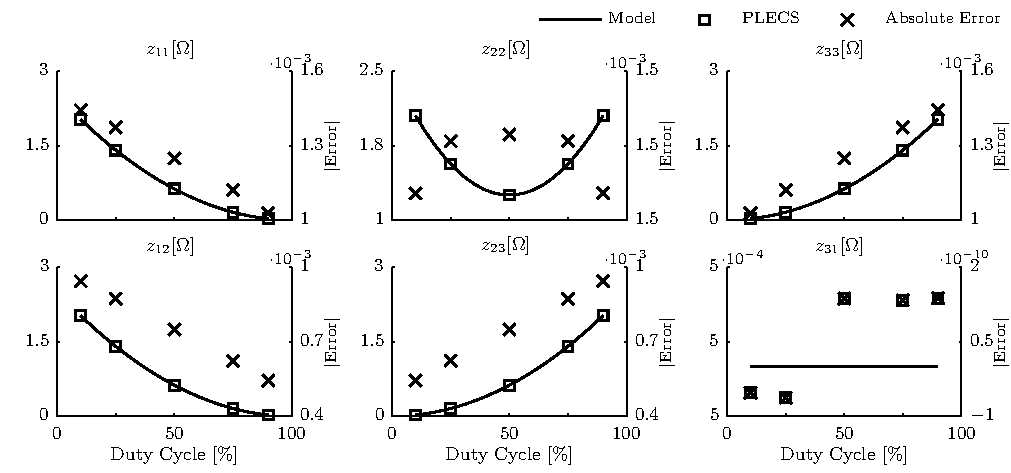
\includegraphics[page=1,width=12cm]{./4_model_validation/APEC_SIM_big}
  \centering
  \caption{SSL comparison between PLECS simulation and the proposed model.}
  \label{fig:sim_ssl}
\end{figure}


\begin{figure}[!h]
  \includegraphics[page=3,width=12cm]{./4_model_validation/APEC_SIM_big}
  \centering
  \caption{FSL comparison between PLECS simulation and the proposed model.}
  \label{fig:sim_fsl}
\end{figure}


\subsection{Experimental results}
An experimental set-up of the converter in was built. The converter uses four MOSFETs TN0104 from Supertex with typical \emph{on}-resistance of 1.5 $\Omega$. Two tantalum electrolytic capacitors of 10$\mu$F have been used as flying capacitors. The circuit was operated at 5kHz and the trans-resistance parameters are measured at different duty cycles. The results are compared with the model and  presented in Fig. \ref{fig:meas_zscc}, it can be seen that the predictions match the measured values with less than 10\% error. All the trans-impedance values with the exception of  parameters $z_{31}$ and $z_{13}$ follow the trend with the duty cycle predicted by the model. $z_{31}$ and $z_{13}$ have a bigger error since these values are much smaller than the rest of the converter parameters and, therefore, more sensitive to the parasitics of the board.

\begin{figure}[!h]
\newcommand\pHeigh{2.750cm}
\newcommand\pWidth{2.500cm}
\centering
	\begin{subfigure}{\textwidth}
		\parbox[b]{0.3250\linewidth}{
		\centering
			\begin{tikzpicture}
    \pgfplotsset{
        width=\pWidth,
        height=\pHeigh,
        scale only axis,
        xlabel near ticks,
        ylabel near ticks,
        scaled y ticks= true ,
        enlarge x limits={0.1},
        enlarge y limits={0.1},
        every tick label/.append style={font=\footnotesize},
        }

	\begin{axis}[
		axis y line*=left,
		axis x line*=bottom,
		xticklabels={,,},
		ylabel = {$r_{scc} [\Omega]$},
		yticklabel style={text width=2.00em,align=right},
		title = {$z_{11}$},
		title style = {
    			font=\footnotesize },
    			at ={(0.75,0.75)},
		]

		\addplot[thin,black,smooth]
    		table [y=y1]{./4_model_validation/c10uF_bis/c10uF_bis_5kHz_Ymdl.dat};

		\addplot[semithick,mark=o,only marks]
    		table [y=y1]{./4_model_validation/c10uF_bis/c10uF_bis_5kHz_Ymeas.dat};

\end{axis}

\end{tikzpicture}

		}
		\parbox[b]{0.3250\linewidth}{
		\centering
			\begin{tikzpicture}
    \pgfplotsset{
        width=\pWidth,
        height=\pHeigh,
        scale only axis,
        xlabel near ticks,
        ylabel near ticks,
        scaled y ticks= true ,
        enlarge x limits={0.1},
        enlarge y limits={0.1},
        every tick label/.append style={font=\footnotesize},
        }

	\begin{axis}[
		axis y line*=left,
		axis x line*=bottom,
		xticklabels={,,},
		yticklabel style={text width=1.50em,align=right},
		title = {$z_{12}$},
		title style = {
    			font=\footnotesize },
    			at ={(0.75,0.75)},
		]

		\addplot[thin,black,smooth]
    		table [y=y4]{./4_model_validation/c10uF_bis/c10uF_bis_5kHz_Ymdl.dat};

		\addplot[semithick,mark=square,only marks]
    		table [y=y4]{./4_model_validation/c10uF_bis/c10uF_bis_5kHz_Ymeas.dat};

	\end{axis}

	\begin{axis}[
		axis y line*=right,
		axis x line=none,
		xticklabels={,,},
		yticklabel pos=right,
		yticklabel style={text width=1.50em,align=left,xshift=-0.50ex},
		enlarge y limits={0.15},
		]

		\addplot[semithick,mark=x,only marks]
    		table [y=y4]{./4_model_validation/c10uF_bis/c10uF_bis_5kHz_Yerr.dat};

	\end{axis}

\end{tikzpicture}

		}
		\parbox[b]{0.3250\linewidth}{
		\centering
			\begin{tikzpicture}
    \pgfplotsset{
        width=\pWidth,
        height=\pHeigh,
        scale only axis,
        xlabel near ticks,
        ylabel near ticks,
        scaled y ticks= true ,
        enlarge x limits={0.1},
        enlarge y limits={0.1},
        every tick label/.append style={font=\footnotesize},
        }

	\begin{axis}[
		axis y line*=left,
		axis x line*=bottom,
		xticklabels={,,},
		yticklabel style={text width=2.00em,align=right},
		title = {$z_{13}$},
		title style = {
    			font=\footnotesize },
    			at ={(0.75,0.75)},
		]

		\addplot[thin,black,smooth]
    		table [y=y7]{./4_model_validation/c10uF_bis/c10uF_bis_5kHz_Ymdl.dat};

		\addplot[semithick,mark=o,only marks]
    		table [y=y7]{./4_model_validation/c10uF_bis/c10uF_bis_5kHz_Ymeas.dat};

\end{axis}

\end{tikzpicture}

		}
	\end{subfigure}

	\begin{subfigure}{\textwidth}
		\parbox[b]{0.3250\linewidth}{
		\centering
			\begin{tikzpicture}
    \pgfplotsset{
        width=\pWidth,
        height=\pHeigh,
        scale only axis,
        xlabel near ticks,
        ylabel near ticks,
        scaled y ticks= true ,
        enlarge x limits={0.1},
        enlarge y limits={0.1},
        every tick label/.append style={font=\footnotesize},
        }

	\begin{axis}[
		axis y line*=left,
		axis x line*=bottom,
		xticklabels={,,},
		ylabel = {$r_{scc} [\Omega]$},
		yticklabel style={text width=1.50em,align=right},
		title = {$z_{21}$},
		title style = {
    			font=\footnotesize },
    			at ={(0.75,0.75)},
		]

		\addplot[thin,black,smooth]
    		table [y=y2]{./4_model_validation/c10uF_bis/c10uF_bis_5kHz_Ymdl.dat};

		\addplot[semithick,mark=square,only marks]
    		table [y=y2]{./4_model_validation/c10uF_bis/c10uF_bis_5kHz_Ymeas.dat};

	\end{axis}

	\begin{axis}[
		axis y line*=right,
		axis x line=none,
		xticklabels={,,},
		yticklabel pos=right,
		yticklabel style={text width=1.50em,align=left,xshift=-0.50ex},
		enlarge y limits={0.15},
		]

		\addplot[semithick,mark=x,only marks]
    		table [y=y2]{./4_model_validation/c10uF_bis/c10uF_bis_5kHz_Yerr.dat};

	\end{axis}

\end{tikzpicture}

		}
		\parbox[b]{0.3250\linewidth}{
		\centering
			\begin{tikzpicture}
    \pgfplotsset{
        width=\pWidth,
        height=\pHeigh,
        scale only axis,
        xlabel near ticks,
        ylabel near ticks,
        scaled y ticks= true ,
        enlarge x limits={0.1},
        enlarge y limits={0.1},
        every tick label/.append style={font=\footnotesize},
        }

	\begin{axis}[
		axis y line*=left,
		axis x line*=bottom,
		xticklabels={,,},
		yticklabel style={text width=2.00em,align=right},
		title = {$z_{22}$},
		title style = {
    			font=\footnotesize },
    			at ={(0.75,0.75)},
		]

		\addplot[thin,black,smooth]
    		table [y=y5]{./4_model_validation/c10uF_bis/c10uF_bis_5kHz_Ymdl.dat};

		\addplot[semithick,mark=o,only marks]
    		table [y=y5]{./4_model_validation/c10uF_bis/c10uF_bis_5kHz_Ymeas.dat};

\end{axis}

\end{tikzpicture}

		}
		\parbox[b]{0.3250\linewidth}{
		\centering
			\begin{tikzpicture}
    \pgfplotsset{
        width=\pWidth,
        height=\pHeigh,
        scale only axis,
        xlabel near ticks,
        ylabel near ticks,
        scaled y ticks= true ,
        enlarge x limits={0.1},
        enlarge y limits={0.1},
        every tick label/.append style={font=\footnotesize},
        }

	\begin{axis}[
		axis y line*=left,
		axis x line*=bottom,
		xticklabels={,,},
		yticklabel style={text width=1.50em,align=right},
		title = {$z_{23}$},
		title style = {
    			font=\footnotesize },
    			at ={(0.75,0.75)},
		]

		\addplot[thin,black,smooth]
    		table [y=y8]{./4_model_validation/c10uF_bis/c10uF_bis_5kHz_Ymdl.dat};

		\addplot[semithick,mark=square,only marks]
    		table [y=y8]{./4_model_validation/c10uF_bis/c10uF_bis_5kHz_Ymeas.dat};

	\end{axis}

	\begin{axis}[
		axis y line*=right,
		axis x line=none,
		xticklabels={,,},
		ylabel = {$\epsilon$},
		yticklabel pos=right,
		yticklabel style={text width=1.50em,align=left,xshift=-0.50ex},
		enlarge y limits={0.15},
		]

		\addplot[semithick,mark=x,only marks]
    		table [y=y8]{./4_model_validation/c10uF_bis/c10uF_bis_5kHz_Yerr.dat};

	\end{axis}

\end{tikzpicture}

		}
	\end{subfigure}

	\begin{subfigure}{\textwidth}
		\parbox[b]{0.3250\linewidth}{
		\centering
			\begin{tikzpicture}
    \pgfplotsset{
        width=\pWidth,
        height=\pHeigh,
        scale only axis,
        xlabel near ticks,
        ylabel near ticks,
        scaled y ticks= true ,
        enlarge x limits={0.1},
        enlarge y limits={0.1},
        every tick label/.append style={font=\footnotesize},
        }

	\begin{axis}[
		axis y line*=left,
		axis x line*=bottom,
		xlabel = {duty cycle},
		ylabel = {$r_{scc} [\Omega]$},
		yticklabel style={text width=1.50em,align=right},
		title = {$z_{31}$},
		title style = {
    			font=\footnotesize },
    			at ={(0.75,0.75)},
		]

		\addplot[thin,black,smooth]
    		table [y=y3]{./4_model_validation/c10uF_bis/c10uF_bis_5kHz_Ymdl.dat};

		\addplot[semithick,mark=square,only marks]
    		table [y=y3]{./4_model_validation/c10uF_bis/c10uF_bis_5kHz_Ymeas.dat};

	\end{axis}

	\begin{axis}[
		axis y line*=right,
		axis x line=none,
		yticklabel pos=right,
		yticklabel style={text width=1.50em,align=left,xshift=-0.50ex},
		enlarge y limits={0.15},
		]

		\addplot[semithick,mark=x,only marks]
    		table [y=y3]{./4_model_validation/c10uF_bis/c10uF_bis_5kHz_Yerr.dat};

	\end{axis}

\end{tikzpicture}

		}
		\parbox[b]{0.3250\linewidth}{
		\centering
			\begin{tikzpicture}
    \pgfplotsset{
        width=\pWidth,
        height=\pHeigh,
        scale only axis,
        xlabel near ticks,
        ylabel near ticks,
        scaled y ticks= true ,
        enlarge x limits={0.1},
        enlarge y limits={0.1},
        every tick label/.append style={font=\footnotesize},
        }

	\begin{axis}[
		axis y line*=left,
		axis x line*=bottom,
		xlabel = {duty cycle},
		yticklabel style={text width=1.50em,align=right},
		title = {$z_{32}$},
		title style = {
    			font=\footnotesize },
    			at ={(0.75,0.75)},
		]

		\addplot[thin,black,smooth]
    		table [y=y6]{./4_model_validation/c10uF_bis/c10uF_bis_5kHz_Ymdl.dat};

		\addplot[semithick,mark=square,only marks]
    		table [y=y6]{./4_model_validation/c10uF_bis/c10uF_bis_5kHz_Ymeas.dat};

	\end{axis}

	\begin{axis}[
		axis y line*=right,
		axis x line=none,
		yticklabel pos=right,
		yticklabel style={text width=1.50em,align=left,xshift=-0.50ex},
		enlarge y limits={0.15},
		]

		\addplot[semithick,mark=x,only marks]
    		table [y=y6]{./4_model_validation/c10uF_bis/c10uF_bis_5kHz_Yerr.dat};

	\end{axis}

\end{tikzpicture}

		}
		\parbox[b]{0.3250\linewidth}{
		\centering
			\begin{tikzpicture}
    \pgfplotsset{
        width=\pWidth,
        height=\pHeigh,
        scale only axis,
        xlabel near ticks,
        ylabel near ticks,
        scaled y ticks= true ,
        enlarge x limits={0.1},
        enlarge y limits={0.1},
        every tick label/.append style={font=\footnotesize},
        }

	\begin{axis}[
		axis y line*=left,
		axis x line*=bottom,
		xlabel = {duty cycle},
		yticklabel style={text width=2.00em,align=right},
		title = {$z_{33}$},
		title style = {
    			font=\footnotesize },
    			at ={(0.75,0.75)},
		]

		\addplot[thin,black,smooth]
    		table [y=y9]{./4_model_validation/c10uF_bis/c10uF_bis_5kHz_Ymdl.dat};

		\addplot[semithick,mark=o,only marks]
    		table [y=y9]{./4_model_validation/c10uF_bis/c10uF_bis_5kHz_Ymeas.dat};

\end{axis}

\end{tikzpicture}

		}
	\end{subfigure}

	\caption[Measured $\mathbf{Z_{scc}}$ from a 2:1 SCC experimental converter.]{Experimental results of the 2:1 SCC, with $f_{sw}=5kHz$. Comparison of the  measured (\emph{$\Box$ markers} ) trans-resistance parameters with the model predicted (\emph{solid line}), and the error ($\epsilon$) between the model and the measures (\emph{x markers}.)}
	\label{}
\end{figure}


%The measured results of the experimental set-up can be improved mounting the circuit in a PCB with less parasitics and operated at higher switching frequencies by using ceramic capacitors instead of the tantalum ones .
\section{Summary}
The presented model is a valuable tool for  modeling a broad range of SCCs, from the classical approach of a single output converter to the new architectures where SCCs are combined with inductors. Unlike the previous models, this method allows to model the behaviour of multiple current loaded outputs, including their coupling relations. The model has been verified with simulations and experiments, and for both cases compares favorably. Since the resulting model is based on analytical expressions; the computation time is dramatically faster than any time-domain based simulator.

At the same time, it has been demonstrated that the original charge flow method was inaccurate in the SSL region, specially when the output capacitor was comparable in size to the flying capacitors. And it was not sensible to the variations of the duty cycle, leading to the wrong estimation of the output resistance of the converter.

The results presented the best accuracy of the model when the converter operates close to the well-defined switching limits, SSL and FSL, with relative errors below $5\%$. When the converter operates in region between the two limits, the relative error can increase up to $20\%$, since the value is approximated from the two asymptotical limits. With regard to the different proposed approximations, results shown the best accuracy using the first proposed approximation of $r_{scc} = \sqrt{r_{ssl}^2 + r_{fsl}^2}$.

\clearpage
\bibliographystyle{plainnat}
\bibliography{references} 